%
% Draft  document radcurv.tex
% Modelling the causes of wool fibre curvature using the Timoshenko equation for curvature of a bimetallic strip subjected to heating
%
 
\documentclass[titlepage]{article}  % Latex2e
\usepackage{graphicx,lscape,subfigure}
\usepackage{tikz}
\usepackage{bm}
\usepackage{textcomp}
 

\title{ Modelling the causes of wool fibre curvature using the Timoshenko equation for curvature of a bimetallic strip subjected to heating}
\author{Neville Jackson}
\date{17 June 2017} 

 
\begin{document} 
 
\maketitle      
\tableofcontents

\clearpage
\section{Acknowledgement}
I wish to thank Dr Jim Watts for his encouragement, and for use of his softness, curvature and diameter data.

\section{Introduction} 
Intrinsic curvature is one of the basic physical properties of a Merino wool fibre.  Each fibre grows with a 'built-in' curved shape which is caused by one side of the fibre growing slighly shorter than the other side. The two portions of the fibre cross section with different growth rates have, in Fine Merino wool, been associated with the two stain-differentiated parts known as paracortex and orthocortex, which exhibit a bilateral symmetric structure in cross section. The paracortex is the shorter growing segment, and ends up on the concave side of the curve (Horio and Kondo(1953)~\cite{hori:53}, Mercer(1954)~\cite{merc:54}). In Strong Merino Wool, and in other non-Merino breeds this is association of stain differentiated cortex with curvature is not always observed.

We confine this study to fine Merino wool, with a bilateral cortical segmentation, and assume that the fibre segments differentiated by staining are the segments which differ in length growth.

The structure of a bi-metal strip is similar to that of a wool fibre. There are two segments ( usually made of two metals of different thermal expansion characteristics) and the strip curves as heat is applied because the lengths of the two segments vary differently with temperature. The analogy with a fibre is not perfect. Bi-metal strips are usually rectangular, fibres are near circular. A fibre emerges from the wool follicle in the skin with the two segments already differeing in length; it is not temperature initiated. It has been suggested (Mercer (1954) ~\cite{merc:54}) that the different lengths of the ortho and para cortex segments in wool is the result of a difference in shortening due to different amounts of keratinization. If this is the case we are looking at a biochemical shortening rather than a thermal expansion.


\section{Bi-metallic strip theory}
We start with a formula from Timoshenko(1925)~\cite{timo:25} which expresses the radius of curvature of a bimetal strip in the following terms
\begin{equation}
\label{eqn:timo}
\rho = \frac{t \left[ 3(1+m)^{2}+(1+mn)(m^{2}+\frac{1}{mn})\right]} {6(\alpha_{2}- \alpha_{1})(T_{H} - T_{C})(1+m)^{2}}
\end{equation}
where
\begin{description}
\item[$\rho$] is the radius of curvature
\item[$t = t_{1} + t_{2}$] is total thickness of the strip, $t_{1},t_{2}$ being the separate thicknesses of the two joined metal strips
\item[$m = t_{1}/t_{2}$] is ratio of thicknesses
\item[$n = E_{1}/E_{2}$] is ratio of Youngs Modulus
\item[$T_{H}\: and\: T_{C}$] are hot and cold temperatures
\item[$\alpha_{1}\: and\: \alpha_{2}$] are coefficients of linear thermal expansion for the two metal strips. $\alpha_{2} > \alpha_{1}$.
\item[$E_{1}\: and\: E_{2}$]are Youngs linear Modulus for metals of the two strips
\end{description}

We can immediately see some things from this formula. There has to be a length difference in the two strips or the radius of curvature $(\rho)$ will be infinity which means the strip will be straight. Also the amount of curvature for a given length difference and thickness depends on the material properties. We can look into these relationships more closely after we put the equation into a form suiteable for a wool fibre.


\section{Application to wool fibres}
 Equation~\ref{eqn:timo} needs some modification to be applicable to a wool fibre. The first and most obvious problem is that we are not studying the effect of temperature change with wool. What we have is a fibre which grows by mitotic division of follicle bulb cells, and the cells differentiate ( and eventually die) as they grow to form 2 different structures within the cortex termed para and ortho cortex. Differentiation follows a slightly different path (or perhaps proceeds for a different length of time) in the two cortical segments. The paracortex ends up shorter, less dye accessible, and differs in microfibril structure as seen in the electron microscope, compared to the paracortex. It has been suggested that different amounts of keratinisation are responsible for different amounts of shorteneing ( and perhaps different Youngs Modulus) of the two segments. So we are probably dealing with different biochemical shortenings, rather than different thermal expansions. To deal with that we need to modify the part of equation~\ref{eqn:timo} which says $(\alpha_{2}- \alpha_{1})(T_{H} - T_{C})$ . We aproach that as follows.

  Those coefficients of linear thermal expansion ($\alpha_{1}$ and $\alpha_{2}$) are increase in length divided by original length per unit rise in temperature. So they are proportional increases in length per unit rise in temperature. To define an analagous quantity for a growing wool fibre we take a short length of fibre which is imagined to be initially straight, as in Figure~\ref{fig:fibre}, of length $\Delta L$ and grown over a time interval $\Delta T$.
%\documentclass{article}
%\usepackage{graphicx,subfigure}
%\begin{document}

\begin{figure}[!h]
  \centering
  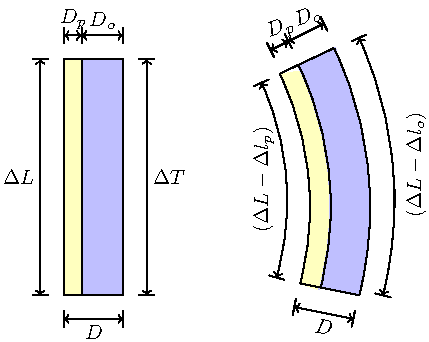
\includegraphics[width=0.9\textwidth]{fibre.pdf}
  \caption{Short lengths of fibre showing the initially straight and curved positions due to differential shortening of the para and ortho cortex segments, which are coloured yellow and blue respectively}
  \label{fig:fibre}
\end{figure}

%\end{document}


 Let diameter $D = Do + Dp$, $D_{o}$ and $D_{p}$ being the thicknesses of the ortho and para cortes segments. Over  the time interval $\Delta T$ and while the short piece of fibre is growing the para and ortho cortex segmnents shrink in length by $\Delta L_{p}$ and $\Delta L_{o}$ respectively, causing the fibre to curve. We can now define the coefficients of  biochemical shrinkage for the fibre as 
\begin{eqnarray*}
 \lambda_{p} & = & \frac{1}{\Delta L} \frac{\Delta L_{p}}{\Delta T} \\
 \lambda_{o} & = & \frac{1}{\Delta L} \frac{\Delta L_{o}}{\Delta T}
\end{eqnarray*}
so the difference becomes
\begin{displaymath}
  (\lambda_{o} - \lambda_{p}) = \frac{1}{\Delta L} \left[ \frac{\Delta L_{o}}{\Delta T} - \frac{\Delta L_{p}}{\Delta T} \right]
\end{displaymath}
and this would define a difference in biochemical shrinkage coefficients for a time interval of $\Delta T$, so it would be in units of $time^{-1}$.

  We now have to consider the $(T_{H} - T_{C})$ term in equation~\ref{eqn:timo}. It is the temperature difference, so it corresponds to our time interval $\Delta T$ for the fibre growth. To get our difference in biochemical shrinkage coefficients into a unitless quantity we have to multiply it by $\Delta T$ as follows
\begin{eqnarray*}
 \lambda & = & (\lambda_{o} - \lambda_{p}) \Delta T \\
        & = & \frac{\Delta T}{\Delta L}\left[ \frac{\Delta L_{o}}{\Delta T} - \frac{\Delta L_{p}}{\Delta T} \right] \\
        & = & \frac{1}{\frac{\Delta L}{\Delta T}} \left[ \frac{\Delta L_{o}}{\Delta T} - \frac{\Delta L_{p}}{\Delta T} \right]
\end{eqnarray*}
so we reduce the whole of  $(\alpha_{2}- \alpha_{1})(T_{H} - T_{C})$ in equation~\ref{eqn:timo} to one parameter $\lambda$, which is a unitless quantity expressed as the difference in shrinkage rate of the two cortex segments as a proportion of the length growth rate of the fibre. Note that $\lambda$ is defined as the difference in shrinkage that would occur if the two segments were not joined into a fibre, in the same manner that the coefficients of thermal expansion are defined for a bimetal strip. The differenece in length actually observed in a curved fibre depends on the amount by which the fibre resists bending.

It is also possible to cancel out the $\Delta T$'s in the equation for $\lambda$ and get $\lambda = \frac{\Delta L_{o} - \Delta L_{p}}{\Delta L}$, which is a differential equation. This form is not likely to be particularly enlightening is the wool case.

 We will change a few other things in equation~\ref{eqn:timo} just to  make a more wool-friendly notation. We shall use $D$ instead of $t$ for total thickness of the fibre, and we shall let $D = D_{p} + D_{o}$ where $D_{p}$ and $D_{o}$ are the two thicknesses of the para and ortho cortex segments, measured perpendicular to the chord separating the two segments.  A bimetal stip is usually made from metal 'flat' sections of equal width, so that the relative thichnesses are the same as the relative cross sectional areas. This is not the case for an approximately circular fibre - the two segments are half-moon shaped.One normally measures para and ortho cortex in wool sections as percentages of area. A ratio of percentages of area is not the same as a ratio of thicknesses for wool. It is not clear which to use for parameter $m$, but we have opted to stay with the ratio of thicknesses, on the grounds that bending strength depends on thickness in the direction of bending, not on area. The problem of converting percentage area measurements to thickneses will be dealt with in a later section.

We want the answer $\rho$ to be in $mm$ units, so with $D$ in microns, we introduce the factor $10^{-3}$

Finally we shall change radius of curvature from $\rho$ to $R$ and note that $R$ will be in units of $mm$.

With these modification we rewrite equation\ref{eqn:timo} for a growing wool fibre as follows
\begin{equation}
\label{eqn:timowool}
R = \left[ \frac{10^{-3}D}{\lambda} \right] \frac{ 3(1+m)^{2}+(1+mn)(m^{2}+\frac{1}{mn})} {6(1+m)^{2}}
\end{equation}
there has been some rearrangement, with the fraction $\frac{10^{-3}D}{\lambda}$ separated from the remainder so that the first term represents physical fibre measurements and the second the properties of the fibre material.

We summarize the new wool fibre notation below
\begin{description}
\item[$R$] is the radius of curvature in $mm$ units
\item[$D = D_{p} + D_{o}$] is diameter of the fibre, $D_{p},D_{o}$ being the separate diameters of the para nd ortho cortex segments
\item[$m = D_{p}/D_{o}$] is ratio of diameters of para and ortho cortex
\item[$n = E_{p}/E_{o}$] is ratio of Youngs Modulus or para and ortho cortex
\item[$E_{p}\: and\: E_{o}$]are Youngs linear Modulus for para and ortho cortex. Youngs modulus for wool is normally in GPa units $(kN/mm^{2})$. A typical value is about 1.4 and there is no information on whether it varies between para and ortho cortex.
\item[$\lambda$] is the difference in shrinkage rates of ortho and para cortex as a proportion of the fibre length growth rate
\end{description}

A number of interpretations of equation~\ref{eqn:timowool} are immediately obvious.
\begin{itemize}
\item for a given $\lambda$ and given material properties curvature is directly proportional to fibre diameter. This is the basis of the observed relationship between crimp ( or quality number) and diameter. It can also be seen that the relationship will not be perfect if any of the other parameters vary.
\item for a given diameter and given material properties curvature is inversely proportional to $\lambda$. If $\lambda = 0$  there is no curvature because $R$ goes to infinity.
\item the material properties ($m$ and $n$) contribute to curvature in a complex way which we shall need to investigate numerically.
\end{itemize}


\section{Numerical examination of the wool fibre curvature equation}
 We first look at the effect of fibre diameter, holding the other parametrs constant at $\lambda = 0.01$, m=1, and n=1. This means a 1 percent difference in length between ortho and para cortex, equal sizes of the para and ortho cortex segments, and equal Young's moduli. The result for diameters ranging from 14 to 22 microns is shown in Figure~\ref{fig:curvd}.
%\documentclass{article}
%\usepackage{graphicx,subfigure}
%\begin{document}

\begin{figure}[!h]
  \centering
  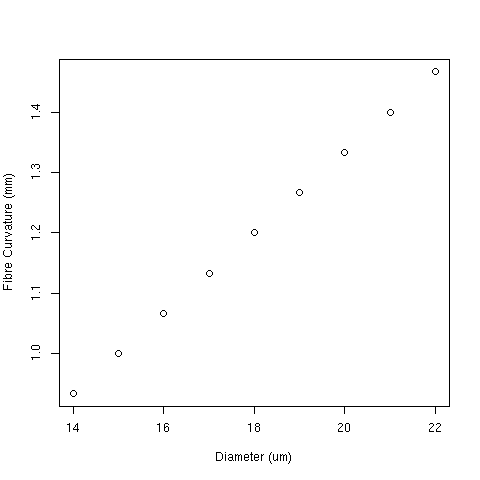
\includegraphics[width=0.9\textwidth]{curvdia.png}
  \caption{Plot of fibre curvature calculated using equation~\ref{eqn:timowool} against $D$ , with the other parameters held constant at  $\lambda=0.01$, $m=1$,  $n=1$.}
  \label{fig:curvd}
\end{figure}

%\end{document}


We see a perfectly linear relationship with curvatures in the range 1.0 to 1.4 mm. That corresponds to a curvature ( in degrees per mm) of 55 to 40 respectively - ie entirely within the expected range for wool.
So curvature is directly proportional to fibre diameter, other things being equal, and the constant of proportion depends in the other parameters. A thick fibre will not bend as much as a thin fibre ( larger radius = bends less) other things being equal.
As we noted above this is the basis of the observed relationship between crimp ( or quality number) and diameter. It can also be seen that the curvature diameter relationship will not be perfect if any of the other parameters vary, and that is why the diameter crimp relationship is imperfect.

 We now look at the effect of changing the relative lengths of the ortho and para cortex segments. We hold the other parameters constant at $D=18$, $m=1$, and $n=1$. We look at a range of valuse of $\lambda$ from 0.005 to 0.04. The result is shown in Figure~\ref{fig:curvlambda}
%\documentclass{article}
%\usepackage{graphicx,subfigure}
%\begin{document}

\begin{figure}[!h]
  \centering
  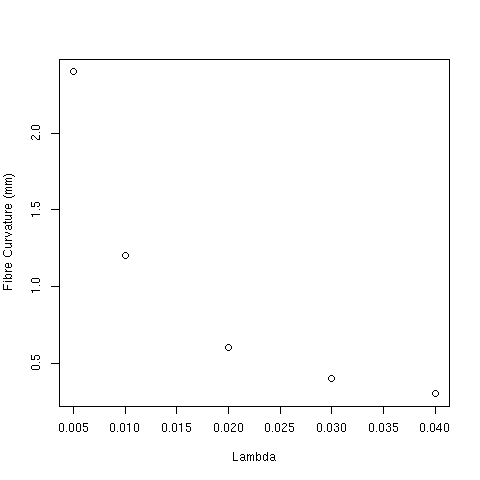
\includegraphics[width=0.9\textwidth]{curvlambda.png}
  \caption{Plot of fibre curvature calculated using equation~\ref{eqn:timowool} against $\lambda$ , with the other parameters held constant at $D=18$, $m=1$,$n=1$.}
  \label{fig:curvlambda}
\end{figure}

%\end{document}


This relationship is nonlinear, because radius is inversely proportional to $\lambda$ in equation~\ref{eqn:timowool}. It is a tyical hyperbolic curve ( like $y=1/x$). The range of $\lambda$ only represents 0.5 percent to 4 percent difference in length between ortho and para cortex. It does not take much length difference to bend a bimetal strip, that is why it is such a sensitive temperature indicator.The same applies to wool. The development paths of ortho and para cortex segments do not have to differ by much to produce a curved fibre. 

We next look at the effect of varying the ratio of para to ortho cortex diameters (m). We vary $m$ over the range 0.1 to 10.0, and hold the other parametrs constant at $D=18$, $\lambda=0.01$, and $n=1$. The result is shown in Figure~\ref{fig:curvm}.
%\documentclass{article}
%\usepackage{graphicx,subfigure}
%\begin{document}

\begin{figure}[!h]
  \centering
  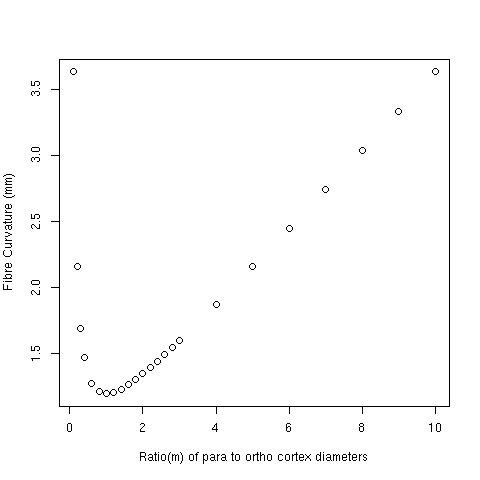
\includegraphics[width=0.9\textwidth]{curvm.png}
  \caption{Plot of fibre curvature calculated using equation~\ref{eqn:timowool} against $m$ , with the other parameters held constant at $D = 18$, $\lambda=0.01$, $n=1$.}
  \label{fig:curvm}
\end{figure}

%\end{document}


This is also very nonlinear, but is quadratic as well as hyperbolic ( ie it is a function of $m$ and $m^{2}$ and $1/m$). There is a minimum radius of curvature at $m=1$, which coincidentally is the value we chose to hold $m$ constant at in the previous graphs. So you get the greatest curvature ( smallest radius) at $m=1$, any deviation from that will increase the radius. In contrast to popular opinion, increasing the proportion of paracortex will only increase the curvature up to the point $m=1$, more than that will reduce the curvature, other things being equal.

We now look at the effect of the ratio($n$) of Youngs moduli  of the para to ortho cortex segments. We vary $n$ over the range 0.1 to 10.0, and hold the other parametrs constant at $D=18$, $\lambda=0.01$, and $m=1$. The result is shown in Figure~\ref{fig:curvn}
%\documentclass{article}
%\usepackage{graphicx,subfigure}
%\begin{document}

\begin{figure}[!h]
  \centering
  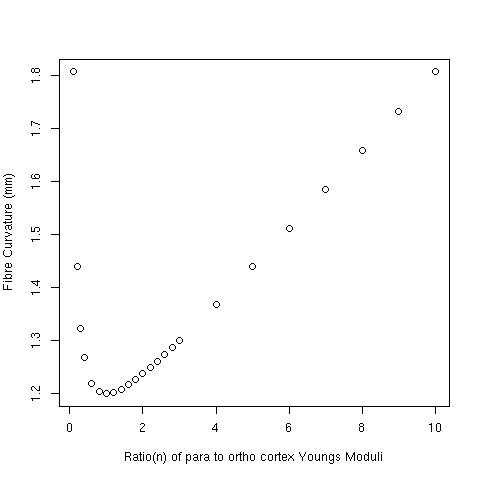
\includegraphics[width=0.9\textwidth]{curvn.png}
  \caption{Plot of fibre curvature calculated using equation~\ref{eqn:timowool} against $n$ , with the other parameters held constant at $D=18$, $\lambda=0.01$, $m=1$.}
  \label{fig:curvn}
\end{figure}

%\end{document}


We get a similar graph to Figure~\ref{fig:curvm}. A curve with a minimum at $n=1$. There are no squared terms in $n$ in equation~\ref{eqn:timowool}, it is combination of a linear term and an hyperbolic term. The range of curvatures is less than in Figure~\ref{fig:curvm}, so $n$ does not affect radius of curvature as strongly as $m$.

Looking at one parametera at a time  does not give the full picture. In particulat $\lambda$ and $n$ will be correlated. We look at this in the next section.

\section{Re-parameterizing $\lambda$ and $n$}
We need to consider that $\lambda$ reflects a difference in the length development of para and ortho cortex, and $n$ reflects the ratio of their elastic strengths. It is likely that both the length diffference and the elasticity ratio depend a single aspect of cortical cell development.

What is known about para and ortho cortex cells is that paracortex cells are slightly smaller in cross section and are slightly longer. This suggests that paracortex cells have simply gone a bit further down the development path towards making fibrils and crosslinking them. So paracortex is simultaneously a bit stronger and a slightly length reduced, compared to orthocortex. We can model this dependence of properties on a single difference in development by reparameterizing as follows.

Define a parameter $K$ which varies from 0 to 1 reflecting the the degree of crosslinking of fibrils in the cortical cells, on an arbitrary scale whene 0 means no crosslinking and 1 means the maximum achievable keratinization. We need one parameter $K_{p}$ for paracortex and another $K_{o}$ for orthocortex, with $K_{p} > K_{o}$. 

Now let the elastic modulus depend on $K$, by some linear proportion so that $E_{p} = k K_{p}$ and $E_{o} = k K_{o}$. We can then reparameterize $n$ as 
\begin{eqnarray*}
n & = & E_{p} / E_{o} \\
  & = & k K_{p} / k K_{o} \\
  & = & K_{p} / K_{o}
\end{eqnarray*}
 so the constant of proportion cancels out. 

Now let the length shrinkage depend proportionally on $K$, so $\lambda_{p} = \kappa  K_{p}$ and $\lambda_{o} = \kappa  K_{o}$. We can then reparameterize $\lambda$ as
\begin{eqnarray*}
\lambda & = & \kappa ( K_{o} - K_{p}) \\
      & = & -\kappa ( K_{p} - K_{o})
\end{eqnarray*}
so we define $\kappa$ to be negative  and reverse the subtraction so we end up with a positive value for $\lambda$. What is $\kappa$? it is simply the amount of length shrinkage achieved when $K = 1$, or alternatively the regression of length shrinkage on $K$. 

So we end up with 3 parameters ($K_{p}$, $ K_{o}$, and $\kappa$), but $\kappa$ is  not something that will vary between sheep, so we really only have $K_{p}$ and $ K_{o}$. The constant $\kappa$ just sets the shrinkage effect of $K$ so it will be a biological constant.

So let us now see the effect on radius of curvature of varying $K_{p}$ and $ K_{o}$ instead of $\lambda$ and $n$. To do this we simply calculate $\lambda$ and $n$ from $K_{p}$ and $ K_{o}$ and substitute their values in equation~\ref{eqn:timowool}.
We will set a value of $\kappa = -0.03$, determined empirically. This means a maximal 3 percent length shrinkage. For a fibre of diameter $D = 18$ microns, and for parameter $m = 0.5$, we calculate R for a range of values of $K_{p}$ and $K_{p}$ and plot the results in Figure~\ref{fig:curvkp}
%\documentclass{article}
%\usepackage{graphicx,subfigure}
%\begin{document}

\begin{figure}[!h]
  \centering
  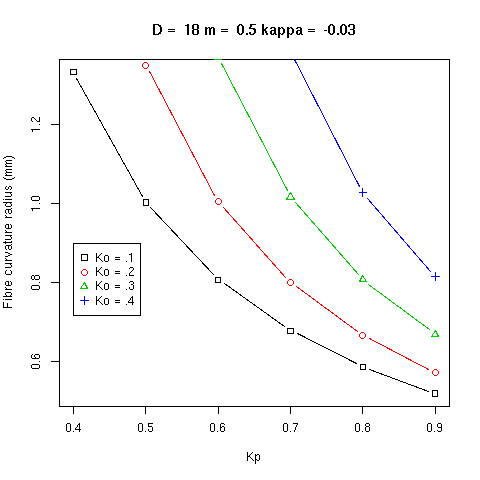
\includegraphics[width=1.0\textwidth]{RvsKpm5.png}
 \caption{Plot of fibre curvature calculated using equation~\ref{eqn:timowool} against $K_{p}$ , with a separate line shown for several values of $K_{o}$, and with the other parameters held constant at $D=18$, $m=0.5$.}
  \label{fig:curvkp}
\end{figure}

%\end{document}


We see a family of curves, one for each stated value of $K_{o}$. From this graph we can read off the fibre properties which would produce a nominal radius of curvature. For example we can get a radius of curvature of $R = 1$ mm, from the combination $K_{p} = 0.5$,$K_{o} = 0.1$, or from the combination $K_{p} = 0.6$,$K_{o} = 0.2$, or from the combination $K_{p} = 0.7$,$K_{o} = 0.3$, etc. 

The combination $K_{p} = 0.5$,$K_{o} = 0.1$ would be a 'soft' fibre and the combination $K_{p} = 0.7$,$K_{o} = 0.3$ would be a 'less soft' fibre. 

If we want more curvature ( smaller radius) we need to change the difference $K_{p} - K_{o}$ to a larger value. For example $K_{p} = 0.6$,$K_{o} = 0.2$ gives $r = 1.0$ , but $K_{p} = 0.6$,$K_{o} = 0.1$ gives $R = 0.8$. 

 We can, of course, substitute for $\lambda$ and $n$ in equation~\ref{eqn:timowool}, instead of numerically. If we do this we get

\begin{equation}
\label{eqn:timowoolop}
R = \left[ \frac{10^{-3}D}{\kappa (K_{p} - K_{o})} \right] \frac{ 3(1+m)^{2}+(1+m \frac{K_{p}}{K_{o}})(m^{2}+\frac{1}{m \frac{K_{p}}{K_{o}}})} {6(1+m)^{2}}
\end{equation}
but this is not very useful as equation~\ref{eqn:timowoolop} does not simplify
readily. It is easier to just do it numerically.

Parameter $m$, the relative thicknesses of para and ortho cortex needs to be looked at in relation to $K_{p}$ and $K_{o}$, but before we can do this we need to relate $m$ to the more usual measurements of percentage area of ortho and para cortex.



\section{Converting between percentages of para and ortho cortex and their thicknesses $D_{p}$ and $D_{o}$.}
The usual way of measuring amounts of para and ortho cortex is as percentages of the cross sectional area of a fibre. However parameter $m$ is defined as the ratio of their thicknesses. We need to develop a corversion formula between the two. This proves to be far more difficult than expected

We start with a circle segmented by a chord as in Figure~\ref{fig:opmeas}.
%\documentclass{article}
%\usepackage{graphicx,subfigure}
%\begin{document}

\begin{figure}[!h]
  \centering
  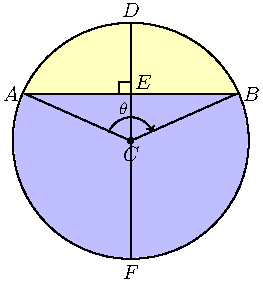
\includegraphics[width=0.7\textwidth]{xsect.pdf}
  \caption{Circle representing a fibre cross-section segmented by a chord AB into para and ortho cortex segments. The para cortex is the yellow segment above chord AB, the orthocortex is the blue segment below chord AB. The parameter $m = D_{p}/D_{o}$ is defined as a ratio of the distance DE to the distance EF. The angle ACB subtended by the chord is referred to as $\theta$ in the text.}
  \label{fig:opmeas}
\end{figure}

%\end{document}


We have a circle of radius $r = AC = CB = CD$ divided by a chord $AB$ into a segment above the chord (which we will let be the para cortex) which has a thickness $D_{p} = DE$, and a segment below the chord ( ortho cortex) which has a thickness $D_{o} = EF$. The diameter if the circle ( representing the fibre diameter) is $D = D_{p} + D_{o} = 2r$. We will let the areas of the para cortex segment be $A_{p}$, and of the ortho cortex segment be $A_{o}$.

The area of a circular segment is given by 
\begin{displaymath}
A = 0.5 r^{2} ( \theta - \sin \theta)
\end{displaymath}
where $\theta$ is the angle subtended by the chord.

So for our wool fibre in Figure~\ref{fig:opmeas}, we have
\begin{eqnarray*}
A_{p} & = & \frac{D^{2}}{8} ( \theta - \sin \theta) \\
A_{o} & = & \frac{D^{2}}{8} ( (2 \pi -\theta) - \sin (2 \pi - \theta)) 
\end{eqnarray*}
and if we convert these areas to percentages of the total cross sectional area $\frac{\pi}{4}D^{2}$ we get 
\begin{eqnarray}
\label{eqn:pop}
P_{p} & = &  \frac{ \theta - \sin \theta}{2  \pi} \\
P_{o} & = & \frac{ (2 \pi -\theta) - \sin (2 \pi - \theta))} {2  \pi}
\end{eqnarray}
The problem is that we cannot turn these equations around and solve for $\theta$ given $P_{p}$ or $P_{o}$.  We need $\theta$ because the formula for $D_{p}$ is in terms of $\theta$, as follows
\begin{eqnarray*}
D_{p} & = & r ( 1 - \cos (\theta/2)) \\
      & = & \frac{D}{2} ( 1 - \cos (\theta/2))
\end{eqnarray*}
and given $D_{p}$ we can get $D_{o}$ and their ratio $m$ as follows
\begin{eqnarray*}
D_{o} & = &  D - D_{p} \\
m     & = & D_{p} / D_{o} \\
      & = & \frac{1-cos(\theta/2)}{1 + cos(\theta/2)}
\end{eqnarray*}

There are two ways of dealing with being unable to solve equation~\ref{eqn:pop} analytically - we can construct a table, or we can solve for $\theta$ numerically with a computer function. We will do both.  First let us make a conversion table. This is shown in Table~\ref{tab:ptom}
%\documentclass{article}
%\usepackage{lscape}
%\begin{document}

\begin{table}[htp]
\centering
\caption{Values of the ratio $m$ and subtended angle $\theta$ for a range of values of percentage of paracortex ina  fibre cross-section}
\label{tab:ptom}
\vspace{0.1in}
\begin{tabular}{|p{0.7in}|p{0.7in}|p{0.7in}|p{0.7in}|}  \hline
    Paracortex & $m$  & $\theta$ & $\theta$  \\ 
  percent & ratio & radians & degrees \\ \hline
   5 & 0.11 & 1.27 & 72.7  \\
  10 & 0.19 & 1.63 & 93.2 \\
  15 & 0.26 & 1.89 & 108.3 \\
  20 & 0.34 & 2.11 & 121.1 \\
  25 & 0.43 & 2.31 & 132.3 \\
  30 & 0.51 & 2.49 & 142.7 \\
  35 & 0.62 & 2.66 & 152.5 \\
  40 & 0.72 & 2.82 & 161.8 \\
  45 & 0.85 & 2.98 & 171.0 \\
  50 & 1.00 & 3.14 & 180.0 \\
  55 & 1.17 & 3.30 & 189.0 \\
  60 & 1.37 & 3.45 & 198.2 \\
  65 & 1.62 & 3.62 & 207.5 \\
  70 & 1.93 & 3.79 & 217.3 \\
  75 & 2.35 & 3.97 & 227.6 \\
  80 & 2.94 & 4.17 & 238.9 \\
  85 & 3.82 & 4.39 & 251.6 \\
  90 & 5.39 & 4.65 & 266.8 \\
  95 & 9.27 & 5.01 & 287.2  \\ \hline
\end{tabular}
\end{table}

%\end{document}

We see that the relation between percent paracortex and $m$ is nonlinear, $M$ increasing sharply at higher values of the percentage of paracortex. The plot in Figure~\ref{fig:ptom} shows this clearly
%\documentclass{article}
%\usepackage{graphicx,subfigure}
%\begin{document}

\begin{figure}[!h]
  \centering
  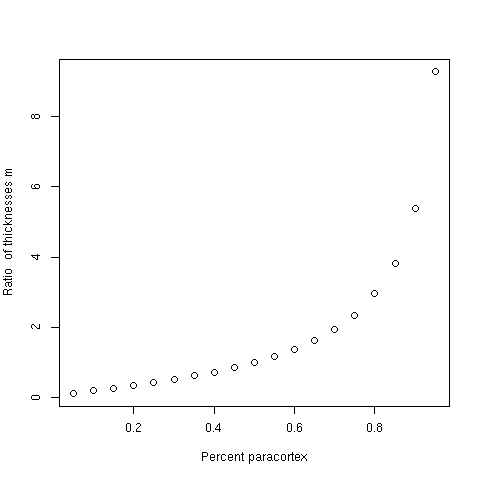
\includegraphics[width=0.8\textwidth]{ptom.png}
  \caption{PLot of percent paracortex against the ratio of thicknesses $(m)$.}
  \label{fig:ptom}
\end{figure}

%\end{document}


However in the region of interest, between about 10 and 50 percent paracortex, the relationship is close to linear.

The computer functions used to compute Table~\ref{tab:ptom} are listed in Appendix A.

We can now have a second look at Figure~\ref{fig:curvkp}  values of $m$ representing percentages of paracortex other than 30 percent ($m = 0.5$). We will look at 40 percent paracortex, corresponding to $m = 0.7$. This is shown in Figure~\ref{fig:curvkp40}.
%\documentclass{article}
%\usepackage{graphicx,subfigure}
%\begin{document}

\begin{figure}[!h]
  \centering
  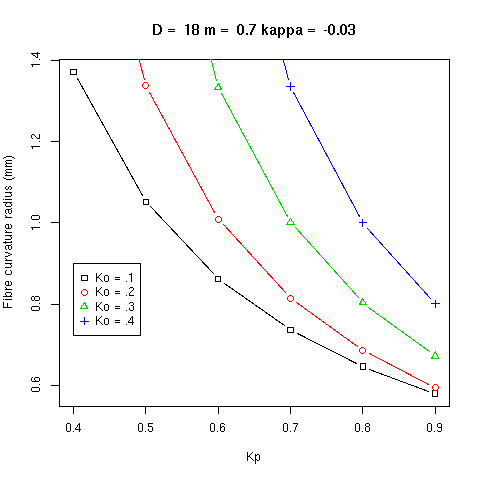
\includegraphics[width=1.0\textwidth]{RvsKpm7.png}
 \caption{Plot of fibre curvature calculated using equation~\ref{eqn:timowool} against $K_{p}$ , with a separate line shown for several values of $K_{o}$, and with the other parameters held constant at $D=18$, $m=0.7$.}
  \label{fig:curvkp40}
\end{figure}

%\end{document}


We see only a slight difference between Figures~\ref{fig:curvkp}  and ~\ref{fig:curvkp40}. The lines are slightly closer in Figure~\ref{fig:curvkp40}.

If we go up to 50 percent paracortex $(m=1.0)$, we get the plot shown in Figure~\ref{fig:curvkp50}
%\documentclass{article}
%\usepackage{graphicx,subfigure}
%\begin{document}

\begin{figure}[!h]
  \centering
  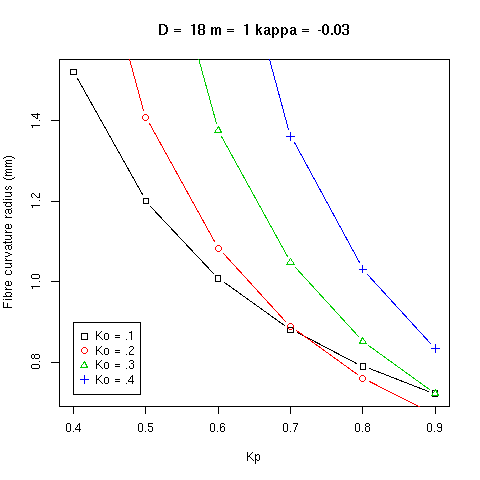
\includegraphics[width=1.0\textwidth]{RvsKpm1.png}
 \caption{Plot of fibre curvature calculated using equation~\ref{eqn:timowool} against $K_{p}$ , with a separate line shown for several values of $K_{o}$, and with the other parameters held constant at $D=18$, $m=1.0$.}
  \label{fig:curvkp50}
\end{figure}

%\end{document}


Now we see an obvious change. The three coloured lines have moved down and to the left so that they intersect the black $(K_{o}=.1)$ line. That means we need a slightly larger value of $K_{p}$ to get the same radius of curvature with 50 percent paracortex, compared to 40 percent paracortex. That makes sense. More paracortex makes the fibre harder to bend so you need to keratinize the paracortex a bit more to make more length shrinkage and hence more bending force.

\section{Single fibre softness}
If we can calculate the radius of curvature $(R)$ of a fibre from its diameter $(D)$ and its material properties $(m, K_{p}, K_{o})$, as in equation~\ref{eqn:timowoolop}, then, in cases where we know the radius of curvature and diameter, maybe we can turn equation~\ref{eqn:timowoolop} around and calculate some type of index of material properties, particularly softness. 

\subsection{Tentative Softness Index}
Let us rearrange the equation to

\begin{equation}
\label{eqn:timosoft}
\frac{R}{10^{-3}D} = \left[ \frac{1}{\kappa (K_{p} - K_{o})} \right] \frac{ 3(1+m)^{2}+(1+m \frac{K_{p}}{K_{o}})(m^{2}+\frac{1}{m \frac{K_{p}}{K_{o}}})} {6(1+m)^{2}}
\end{equation}
We now have all the material properties on the right hand side, and the two traits we might be able to measure ($D$ and $R$ ) on the left hand side. This suggests that $\frac{R}{10^{-3}D}$ might be some sort of an index of softness, not softness of a wool bulk, but softness of a single fibre measured by its resistance to bending.

This is an untested  hypothesis. We need to check it with some actual data. There is not much data available on intrinsic radius of curvature $(R)$, because it has been shown that measurements of curvature of fibres either on snippets or in staples are biased (Watts and Jackson(2016)~\cite{watt:16}). What we are able to get is intrinsic radius of curvature predicted from follicle curvature using the procedure developed by Jackson and Watts(2016)~\cite{jack:16b}. We have calculated $R$ in this way, from follicle curvature, for a set of 340 Merino sheep for which fibre diameter measurements and scores for softness are available.
We then used the calculated $R$ to get
\begin{displaymath}
I = \frac{R}{10^{-3}D}
\end{displaymath}
where $I$ is our "Softness Index" , and compare it to the wool staple softness scores in Figure~\ref{fig:soft}
%\documentclass{article}
%\usepackage{graphicx,subfigure}
%\begin{document}

\begin{figure}[!h]
  \centering
  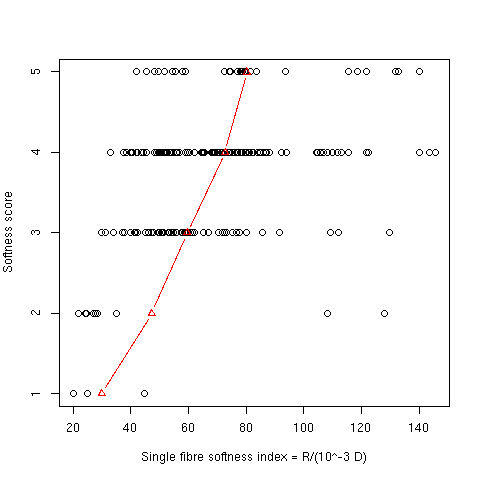
\includegraphics[width=0.9\textwidth]{soft.png}
  \caption{Plot of Softness Index $(I)$ calculated as $R/(10^{-3} D$ against subjective Softness Scores done on wool staples, for 340 Merino sheep in a data set belonging to Dr Jim Watts. The $R$ refers to intrinsic radius of curvature in $mm$ calculated from follicle curvature scores as described in Jackson and Watts(2016)~\cite{jack:16b}, and the $D$ refers to average fibre diameter in microns. The red triangles show the mean Softness Index, at each of the five Softness Scores.}
  \label{fig:soft}
\end{figure}

%\end{document}


 There is a lot of variation in Figure~\ref{fig:soft}, but there is also a definite trend in the means for each softness score ( shown in red ). The actual means of "Softness Index" for each softness score are shown in Table~\ref{tab:soft}.
%\documentclass{article}
%\usepackage{lscape}
%\begin{document}

\begin{table}[htp]
\centering
\caption{Means of Softness Index, Fibre Diameter, and Intrinsic Radius of curvature, for each of the five Softness score levels, for a set of 340 sheep with data belonging to Dr Jim Watts.}
\label{tab:soft}
\vspace{0.1in}
\begin{tabular}{|p{1.0in}|p{1.0in}|p{1.0in}|p{1.0in}|}  \hline
    Softness Score & Mean Softness Index  & Mean Fibre Diameter  & Mean Intrinsic Radius  \\ 
  score & ratio & $\mu m$ & $mm$ \\ \hline
  1 & 29.9 & 18.7 & 0.60 \\
  2 & 47.4 & 20.0 & 0.93 \\
  3 & 59.7 & 18.7 & 1.12 \\
  4 & 72.8 & 18.6 & 1.36 \\
  5 & 80.3 & 18.2 & 1.45  \\ \hline
\end{tabular}
\end{table}

%\end{document}

So the wools scored as softest ( score = 5) have the highest "Softness Index", and the largest intrinsic radius ( ie the least curvature), but do not differ in mean fibre diameter. This suggests that the material properties ( parameters $m$, $K_{p}$ and $K_{o}$) associated with single fibre softness also lead to a large intrinsic radius. That is likely; if $K_{p}$ is a lot larger than $K_{o}$, one will get a hard fibre and a small radius.

We have to be careful comparing softness scores with "Softness Index". Single fibre softness is not the softness of a fibre bulk. The factors affecting compressional properties of a fibre bulk are well known (Chaudri and Whiteley (1968)~\cite{chau:68}). Resistance to compression depends on fibre diameter, crimp frequency, crimp form, and fibre arrangement. A lot of angular fibre contacts - as in a carded wool sample or in a poorly aligned staple -  leads to increased resistance to compression. The measurement of resistance to compression is therefore done on a randomized fibre assembly such as a carded wool sample. Softness scores made on staples will depend partly on fibre arrangement, as well as actual single fibre softness. This may be where some of the variation in Figure~\ref{fig:soft} is arising from. At least for well aligned staples, softness score is probably closely related to single fibre softness. Very soft fibres typically make staples with a 'floppy' characteristic which indicates that the fibres bend easily and are aligned.

The prominence of crimp form in the Chaudri and Whiteley (1968)~\cite{chau:68} paper is interesting. Crimp form is a measure of whether the fibre crimp is helical or planar.  It may be analagous to the distinction between stretched-helix and unfolded-helix crimp made by Jackson and Watts(2016)~\cite{jack:16}. If that is so, then the real effect on compressional resistance or softness is not crimp {\em per se}, but the material properties of the fibre that are responsible for crimp. Unfolded-helix crimp requires a large radius of curvature ( low crimp frequency or curvature) and that in turn requires a less keratinized paracortex, or a smaller difference between para and ortho cortex. So, on that theory, softness is a fibre property, not a bulk property.

Our "Softness Index" $(I)$ is only vaguely supported by the data. There is too much variation within each score grade.

\subsection{The parts of equation~\ref{eqn:timosoft}}
We need to look more closely at equation~\ref{eqn:timosoft} to see if we can interpret each part, and thereby have some confidence in what it is calculating. In particular, the right hand side of equation~\ref{eqn:timosoft} can be broken into two parts. The first
\begin{displaymath}
\frac{1}{\kappa(K_{p} - K_{o})}
\end{displaymath}
represents the reciprocal of the length shrinkage difference between para and ortho cortex. As such, it is a material property, because it depends on $K_{p}$ and $K_{o}$, but it also represents the {\em force} which is causing the fibre to curve.   Not the actual amount of curvature, but what the radius would be if there were no resistance to bending ( ie if the fibre were infinitely soft and thin).

The second part 
\begin{displaymath}
 M = \frac{ 3(1+m)^{2}+(1+m \frac{K_{p}}{K_{o}})(m^{2}+\frac{1}{m \frac{K_{p}}{K_{o}}})} {6(1+m)^{2}}
\end{displaymath}
represents a multiplier which 'corrects' the first part for variations in the bilateral structure of the fibre as specified by $m$ and $\frac{K_{p}}{K_{o}}$. 

Both parts depend in $K_{p}$ and $K_{o}$, the first part depends on their difference, the second part depends on their ratio. We can see this more clearly in Figure~\ref{fig:softparts} where we plot the two parts for a range of values of $K_{p}$ and $K_{o}$.
%\documentclass{article}
%\usepackage{graphicx,subfigure}
%\begin{document}

\begin{figure}[!h]
  \centering
  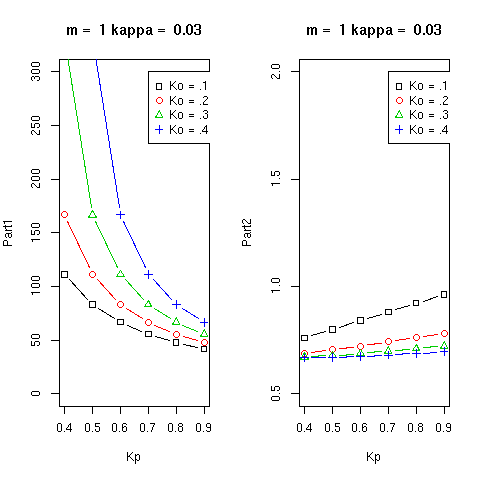
\includegraphics[width=1.1\textwidth]{softparts.png}
  \caption{Plots of the two parts of Softness Index $(I)$ defined in equation~\ref{eqn:timosoft} for a range of values of $K_{p}$ and $K_{o}$.}
  \label{fig:softparts}
\end{figure}

%\end{document}


We see that part1 becomes very large as $K_{p}$ decreases with $K_{o}$ held constant, while part2 varies only a little. A small difference $(K_{p} - K_{o})$ leads to a large part1 and therefore a large "Softness Index".  It would seem that soft fibres have a similar degree of keratinization in the ortho and para segments, and that is why large radius ( small curvature) fibres are soft, other things being equal.


 We can see this more clearly if we go back to equation~\ref{eqn:timowoolop}, which we repeat below
\begin{displaymath}
\label{eqn:timorepeat}
R = \left[ \frac{10^{-3}D}{\kappa (K_{p} - K_{o})} \right] \frac{ 3(1+m)^{2}+(1+m \frac{K_{p}}{K_{o}})(m^{2}+\frac{1}{m \frac{K_{p}}{K_{o}}})} {6(1+m)^{2}}
\end{displaymath}
so we can now see that the first term on the right hand side 
\begin{displaymath}
\left[ \frac{10^{-3}D}{\kappa (K_{p} - K_{o})} \right]
\end{displaymath}
will be in $mm$ units and will represent the actual radius of curvature in $mm$ that would occur if the bending force caused by the length difference $\kappa(K_{p} - K_{o})$ encountered some vaguely defined average resistance to bending. We will call this term $R_{1}$. $R_{1}$ approaches a minimum as the difference $(K_{p} - K_{o})$ approaches $1$. The minimum value is $\frac{10^{-3}D}{\kappa}$, so in setting up $\kappa = .03$ we have defined the minimum radius for a 30 micron fibre to be $ 1mm$, and for a 20 micron fibre $0.66mm$, etc. So when $(K_{p} - K_{o})$ is less than $1$ , what $R_{1}$ defines is the minumum radius achievable with that value of $(K_{p} - K_{o})$. 

This leaves the second term on the right hand side,
\begin{displaymath}
M = \frac{ 3(1+m)^{2}+(1+m \frac{K_{p}}{K_{o}})(m^{2}+\frac{1}{m \frac{K_{p}}{K_{o}}})} {6(1+m)^{2}}
\end{displaymath}
which is a unitless ratio that varies between about 0.6 and about 1, a minimum value of about 0.6 is obtained when $m=0.5$, that is with 30 percent para cortex.
What this seems to mean is that the second term is a multiplier which varies the radius of curvature estimate from the first term, to allow for the bilateral asymmetery of the fibre, both the bilateral proportions, and their relative bending properties.

So where does that leave us with softness. The indication is that our "Softness Index" is probably not quite correct.  It does not separate the bending force due to the length differnce betweeen para and ortho cortex from the material properties. The variability within each softness score in Figure~\ref{fig:soft} is probably variation in $(K_{p} - K_{o})$. We can do no better because only $R$ and $D$ are likely to be available as measurements.

\subsection{Separating bending force from material properties}
We need to think outside of the Timoshenko equation. A given length difference between para and ortho cortex has the potential to lead to a certain minimum radius of curvature, in an hypothetical situation where the material of the fibre offers zero resistance to bending, so that no stress remains within the fibre and it is able to fully realize its potential to curve. 

We can calculate this minimum potential radius of curvature from the simple geometry of a bent section of fibre. Figure~\ref{fig:rmin} shows a short section of fibre with the lengths of para and ortho cortex segments shown as $l_{p}$ and $l_{o}$, the lengths of their centrelines.
%\documentclass{article}
%\usepackage{graphicx,subfigure}
%\begin{document}

\begin{figure}[!h]
  \centering
  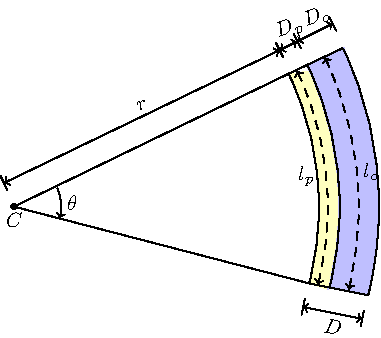
\includegraphics[width=0.9\textwidth]{rmin.pdf}
  \caption{A curved length of fibre with its radius of curvature centred at point $C$. The para cortex is the yellow segment, and its length is shown as the dotted centreline length $l_{p}$. The orthocortex is the blue segment and its length is shown as the dotted centreline length $l_{o}$. The radius of the inner edge of the curved fibre is $r$. The angle subtended at the centre of itsradius of curvature is $\theta$.}
  \label{fig:rmin}
\end{figure}

%\end{document}


The bent snippet in Figure~\ref{fig:rmin} has a radius of curvature of its inner edge shown as $r$, and we define the radius of curvature of the whole snippet to be $R_{min} = r + \frac{D}{2}$.  In other words, the snippet drawn in Figure~\ref{fig:rmin} is at its minimum potential radius of curvature, with the length difference $(l_{p} - l_{o})$ being fully expressed as curvature.

The length of an arc is the product of its radius and the subtended angle, so we can write
\begin{eqnarray*}
R_{p} & = & r + \frac{D_{p}}{2} \\
R_{o} & = & r + \frac{D_{o}}{2} \\
l_{p} & = & R_{p} \theta \\
l_{o} & = & R_{o} \theta \\
l_{min} & = & R_{min} \theta
\end{eqnarray*}
where $l_{min}$ is the length of the centreline of the whole snippet.

We can now write equations for $l_{p}$ and $l_{o}$ as
\begin{eqnarray*}
l_{p} & = & \left( r  + \frac{D_{p}}{2} \right) \theta  \\
l_{o} & = & \left( r  + D_{p} + \frac{D_{o}}{2} \right) \theta
\end{eqnarray*}
and we can subtract them to get
\begin{displaymath}
l_{p} - l_{o} = \frac{1}{2}(D_{o} + D_{p})) \theta
\end{displaymath}
From there we can divide by the average length of the snippet to get the proportional or percentage difference in lengths of ortho and para cortes as
\begin{eqnarray*}
\frac{l_{p} - l_{o}}{l_{min}} & =  & \frac{\frac{1}{2}(D_{o} + D_{p}) \theta}{R_{min} \theta} \\
       & = & \frac{\frac{1}{2}(D_{o} + D_{p})}{R_{min}} \\
       & = & \frac{\frac{1}{2}10^{-3}D}{R_{min}}
\end{eqnarray*}
putting diameter $(10^{-3}D)$ in $mm$ units

So, now that we have the proportional difference in lengths of ortho and para cortex in terms of $D$ and $R_{min}$, we can substitute it for the term $\kappa (K_{p} = K_{o})$ in the Timoshenko equation, to get 

\begin{eqnarray*}
R & = & \left[ \frac{10^{-3}D}{\kappa (K_{p} - K_{o})} \right] \frac{ 3(1+m)^{2}+(1+m \frac{K_{p}}{K_{o}})(m^{2}+\frac{1}{m \frac{K_{p}}{K_{o}}})} {6(1+m)^{2}} \\
  & = &  \left[ \frac{10^{-3}D} {\frac{\frac{1}{2}10^{-3}D}{R_{min}} } \right] M \\
  & = & 2 R_{min} M
\end{eqnarray*}
letting $M$ stand for the large fraction on the right which represents material properties.

We might finally move $R_{min}$ to the left side of the equation, so that we end up with a formula for the ratio of actual radius curvature $(R)$ to minimum potential radius of curvature $(R_{min})$, as follows
\begin{equation}
\label{eqn:softratio}
\frac{R}{2 R_{min}} =  M
\end{equation}
 We will call equation~\ref{eqn:softratio} "Material Softness Ratio". We note that it depends solely on $M$, in other words on $m$, and $\frac{K_{p}}{K_{o}}$, but not on $(K_{o} - K_{p})$.  $M$ is referred to as 'part2' in the previous section, and its value is graphed in Figure~\ref{fig:softparts}, whence we see that it has values between $0.5$ and $1.0$.  

One might think that fibre diameter $D$ is missing from our "Material Softness Ratio", because $D$ cancelled out in our equations. That is correct. The softness of a material is independent of its thickness. Think of soft versus hard licquorice; the thickness of the liquorice pieces has no effect on their 'biting softness'. The same applies to fibres, but the parameter $M$ is a complicated fraction because the fibre material is not homogeneous. 

We have to remember that our "Material Softness Ratio" is defined in terms of radius, not curvature. For a very 'soft' fibre, $R$ will approach $R_{min}$ so our ratio will be small ( approaching $0.5$ in the limit). So a small number indicates 'soft' by our definition of "Material Softness Ratio". 

"Material Softness Ratio" is not going to be of practical use, unless we know $m$, and $\frac{K_{p}}{K_{o}}$. What it does is demonstrate why our "Softness Index" calculated from $R$ and $D$ is not the softness of the fibre material.

\subsection{Fibre bending softness}
In the previous section we defined the "Material Softness" or "Intrinsic Softness" of a fibre. Now we want to separate the component of the Timoshenko equation which represents resistance to bending, which we might call "Fibre bending softness". 

To see what governs resistance to bending, we rearrange equation~\ref{eqn:timowoolop} again to get

\begin{equation}
\label{eqn:timowoolbend}
R = \left[ \frac{1}{\kappa (K_{p} - K_{o})} \right] \left[ 10^{-3}D M \right]
\end{equation}
now the first term on the right hand side represents 'degree of bending due to para/ortho length difference' and the second term represents 'degree to which the fibre resists bending'.

So the second term $10^{-3}D M$ is "Fibre Bending Softness", and again it is on an inverse scale, a small number is less resistance to bending, that is 'softer'. Again, "Fibre bending softness" is not going to be of practical use, unless we know $M$. It does demonstrate that our tentative "Softness Index" is not fibre bending softness.


\subsection{Summary of softness investigation}
We started with  equation~\ref{eqn:timowool} for radius of curvature, and saw that if we shifted $10^{-3}D$ to the left side of the equation we ended up with $\frac{R}{10^{-3}D}$ on the left and all the material properties parameters on the right ( equation~\ref{eqn:timosoft}). We the 'guessed' that $\frac{R}{10^{-3}D}$ might be some sort of "Softness Index", and because $R$ and $D$ are measurable we were able to compute $\frac{R}{10^{-3}D}$ for some sheep and compare it with some Softness scores done on staples. There was a correlation, but there was a lot of noise too.

Then we looked at equation~\ref{eqn:timowool} and decided that the term $\frac{10^{-3}D}{\kappa(K_{p} - K_{o})}$ represented the radius of curvature produced by a length difference of $\kappa(K_{p} - K_{o})$ between para and ortho cortex , not the actual radius of curvature, but the potential radius ignoring any resistance to bending arising from the material properties of the fibre. The remaining term on the right hand side of equation~\ref{eqn:timosoft}, which we called $M$ represents the way the material properties modify the potential curvature before it becomes actual. This suggests that perhaps softness should be obtained as the ratio of actual to potential radius of curvature, given by $\frac{R \kappa(K_{p} - K_{o})}{10^{-3}D} = M$

We needed to clarify what this 'potential radius' actually represents, so we went to the simple geometry of a curved fibre,  and showed that the proportional difference in length represented by $\kappa(K_{p} - K_{o})$ became $\frac{10^{-3}D}{2 R_{min}}$ if the fibre curved without resistance to bending. Substituting this in equation~\ref{eqn:timowool}  and rearranging led to $\frac{R}{2 R_{min}} = M$, which shows that our 'potential radius' above is actually $2 R_{min}$. We now have confidence that $\frac{R}{2 R_{min}} = M$  is the "Material Softness" of the fibre.

Finally we were able to see that resistance of the fibre to bending, which we might call "Fibre Bending Softness" depends on both fibre diameter $D$ and the material softness pararmeter $M$. So we were able to write $R \kappa(K_{p} - K_{o}) = 10^{-3}D M$ so that "Fibre bending Softness" is a function of radius $R$ and the para-ortho length difference.

We should note that neither "Fibre Material Softness" nor "Fibre Bending Softness" is the same thing as "Smoothness". Smoothness depends on surface characteristics of the fibre; the size and protrusion of scales forming the cuticle. We have only looked at the fibre cortex structure, and have therefore assumend that the cuticle has little effect on fibre curvature. The cuticle scales are about 2 micron thick, and therefore contribute about 4 microns to fibre diameter. Their contribution to material properties is unknown, but we do know that the scales are highly keratinized, like the paracortex.

\section{Discussion}
We have achieved a precise understanding of radius of curvature. It depends on 
the following
\begin{itemize}
\item fibre diameter
\item the difference $(K_{p} - K_{o})$ between the degrees of keratinization of the para and ortho cortex segments
\item the ratio $\frac{K_{p}}{K_{o}}$ of the degrees of keratinization of the para and orthocortex segements
\item the ratio $\frac{D_{p}}{D_{o}} = m$ of the thicknesses of the para and ortho cortex segments
\end{itemize}
The way these components combine is complex. In particular dependence of both a difference and a ratio is difficult to comprehend. It is best handled by plotting numerical results, and this is what we have attempted.

How much softness contributes to and is therefore correlated with radius of curvature is a much more difficult topic. All of the above radius of curvature components , except $(K_{p} - K_{o})$, are involved in fibre bending softness, but softness is not just radius of curvature. Fibre bending softness can be decomposed into fibre diameter and fibre material softness. Fibre material softness depends only on the parameter $M$. We have shown that to properly make a separation of softness and radius, we need to know either minimum potential radius, or the parameters $m$ and $\frac{K_{p}}{K_{o}}$.  

The way the various parameters interact to determine both radius of curvature and fibre bending softness has been summarised in Figure~\ref{fig:curvdia} as a flowchart diagram.
% Graphic for TeX using PGF
% Title: /home/nevj/common/Dia/Diagram8.dia
% Creator: Dia v0.97.3
% CreationDate: Sun Jun 18 21:03:20 2017
% For: nevj
%\documentclass{article}
%\usepackage{graphicx,lscape}
% \usepackage{tikz}
%\begin{document}
\begin{landscape}
\begin{figure}[!h]
  \centering
\label{fig:curvdia}

% The following commands are not supported in PSTricks at present
% We define them conditionally, so when they are implemented,
% this pgf file will use them.
\ifx\du\undefined
  \newlength{\du}
\fi
\setlength{\du}{15\unitlength}
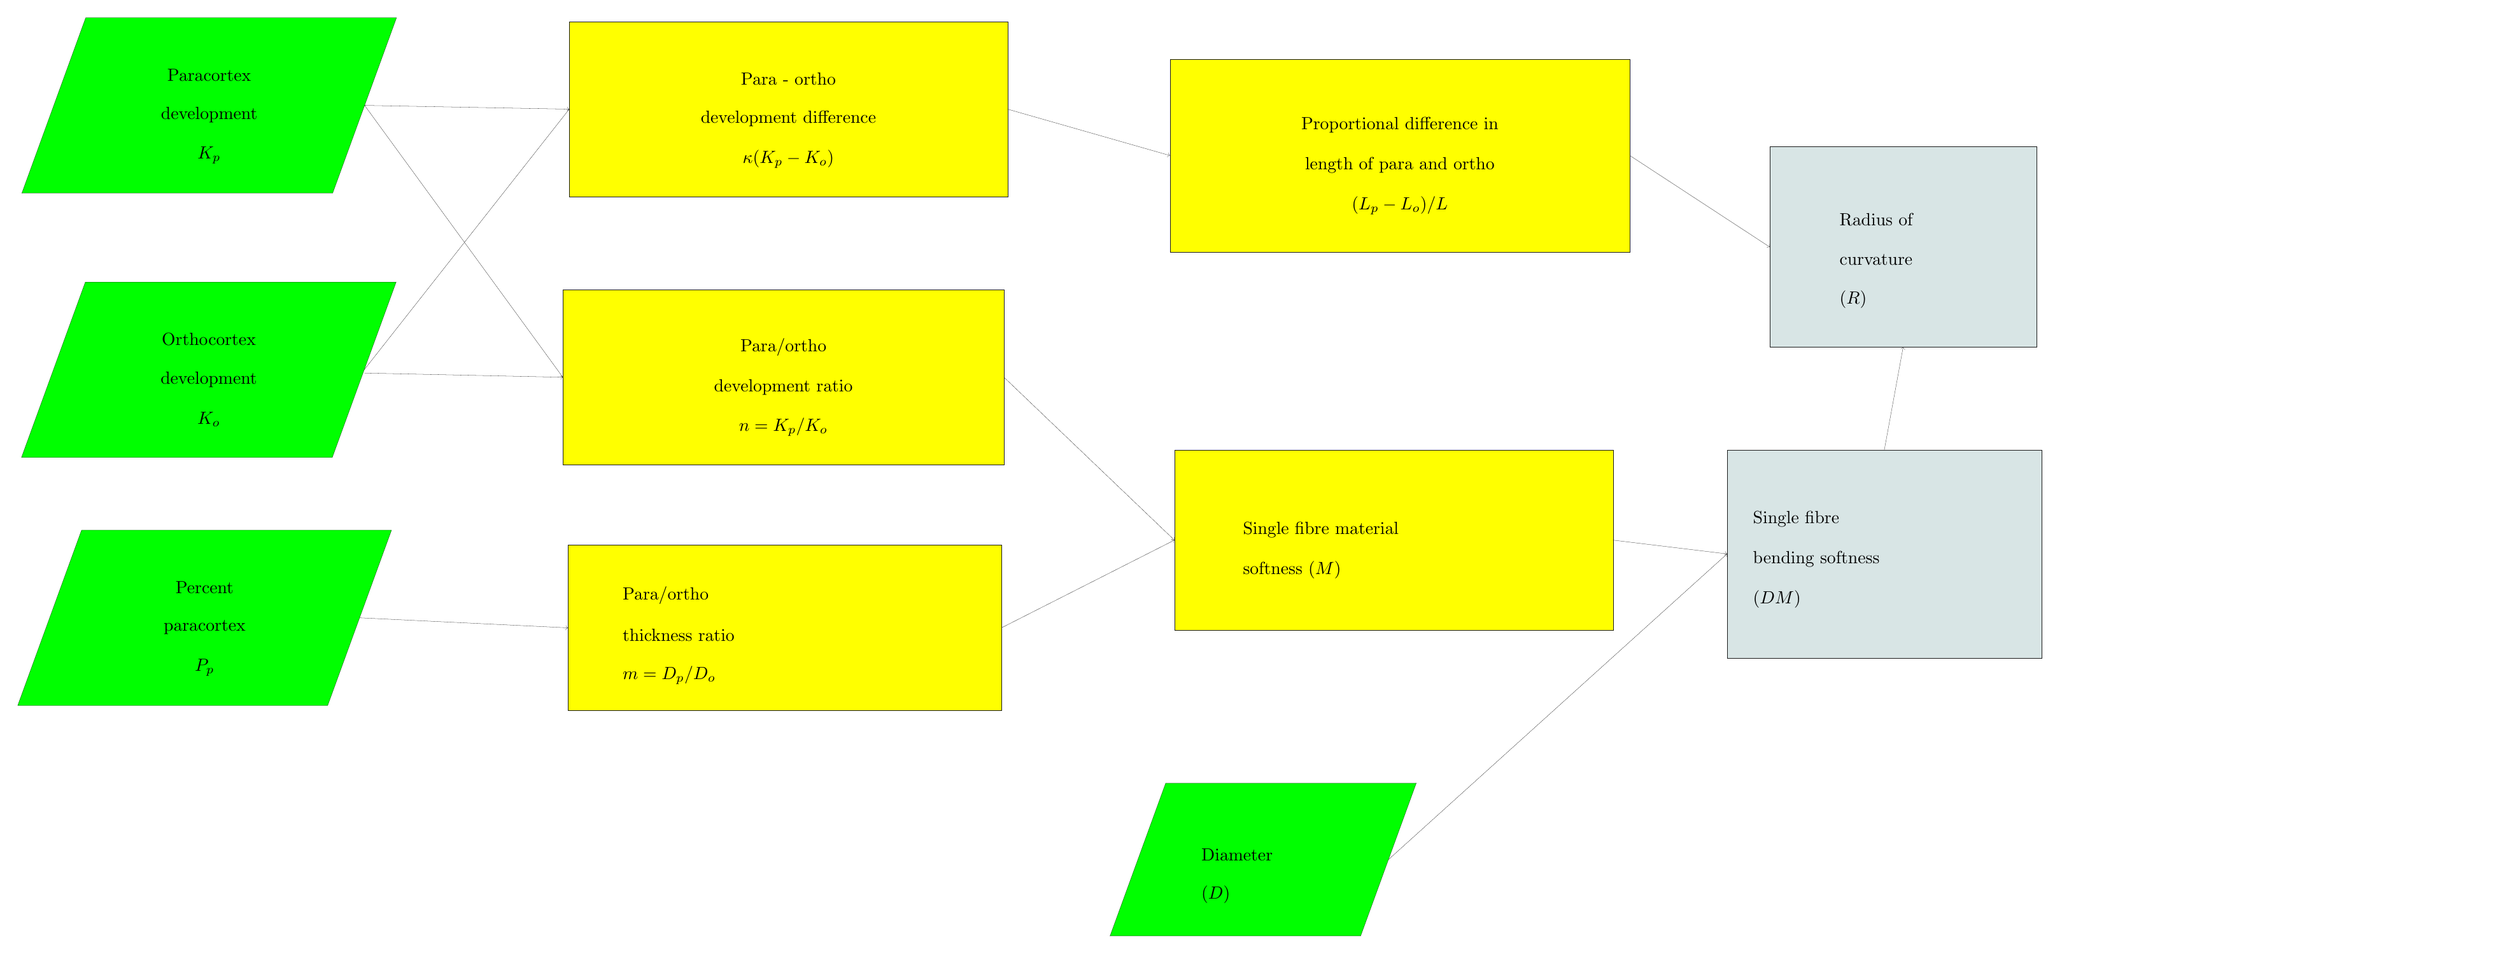
\begin{tikzpicture}
\pgftransformxscale{1.000000}
\pgftransformyscale{-1.000000}
\definecolor{dialinecolor}{rgb}{0.000000, 0.000000, 0.000000}
\pgfsetstrokecolor{dialinecolor}
\definecolor{dialinecolor}{rgb}{1.000000, 1.000000, 1.000000}
\pgfsetfillcolor{dialinecolor}
\definecolor{dialinecolor}{rgb}{0.000000, 1.000000, 0.000000}
\pgfsetfillcolor{dialinecolor}
\fill (1.481656\du,1.475000\du)--(7.682684\du,1.475000\du)--(6.408789\du,4.975000\du)--(0.207760\du,4.975000\du)--cycle;
\pgfsetlinewidth{0.100000\du}
\pgfsetdash{}{0pt}
\pgfsetdash{}{0pt}
\pgfsetmiterjoin
\definecolor{dialinecolor}{rgb}{0.101961, 0.101961, 0.101961}
\pgfsetstrokecolor{dialinecolor}
\draw (1.481656\du,1.475000\du)--(7.682684\du,1.475000\du)--(6.408789\du,4.975000\du)--(0.207760\du,4.975000\du)--cycle;
% setfont left to latex
\definecolor{dialinecolor}{rgb}{0.101961, 0.101961, 0.101961}
\pgfsetstrokecolor{dialinecolor}
\node at (3.945222\du,2.620000\du){Paracortex};
% setfont left to latex
\definecolor{dialinecolor}{rgb}{0.101961, 0.101961, 0.101961}
\pgfsetstrokecolor{dialinecolor}
\node at (3.945222\du,3.420000\du){development};
% setfont left to latex
\definecolor{dialinecolor}{rgb}{0.101961, 0.101961, 0.101961}
\pgfsetstrokecolor{dialinecolor}
\node at (3.945222\du,4.220000\du){$K_{p}$};
\definecolor{dialinecolor}{rgb}{0.000000, 1.000000, 0.000000}
\pgfsetfillcolor{dialinecolor}
\fill (1.474072\du,6.750000\du)--(7.675100\du,6.750000\du)--(6.401205\du,10.250000\du)--(0.200176\du,10.250000\du)--cycle;
\pgfsetlinewidth{0.100000\du}
\pgfsetdash{}{0pt}
\pgfsetdash{}{0pt}
\pgfsetmiterjoin
\definecolor{dialinecolor}{rgb}{0.101961, 0.101961, 0.101961}
\pgfsetstrokecolor{dialinecolor}
\draw (1.474072\du,6.750000\du)--(7.675100\du,6.750000\du)--(6.401205\du,10.250000\du)--(0.200176\du,10.250000\du)--cycle;
% setfont left to latex
\definecolor{dialinecolor}{rgb}{0.101961, 0.101961, 0.101961}
\pgfsetstrokecolor{dialinecolor}
\node at (3.937638\du,7.895000\du){Orthocortex};
% setfont left to latex
\definecolor{dialinecolor}{rgb}{0.101961, 0.101961, 0.101961}
\pgfsetstrokecolor{dialinecolor}
\node at (3.937638\du,8.695000\du){development};
% setfont left to latex
\definecolor{dialinecolor}{rgb}{0.101961, 0.101961, 0.101961}
\pgfsetstrokecolor{dialinecolor}
\node at (3.937638\du,9.495000\du){$K_{o}$};
\definecolor{dialinecolor}{rgb}{0.000000, 1.000000, 0.000000}
\pgfsetfillcolor{dialinecolor}
\fill (1.398996\du,11.700000\du)--(7.582683\du,11.700000\du)--(6.308787\du,15.200000\du)--(0.125100\du,15.200000\du)--cycle;
\pgfsetlinewidth{0.100000\du}
\pgfsetdash{}{0pt}
\pgfsetdash{}{0pt}
\pgfsetmiterjoin
\definecolor{dialinecolor}{rgb}{0.101961, 0.101961, 0.101961}
\pgfsetstrokecolor{dialinecolor}
\draw (1.398996\du,11.700000\du)--(7.582683\du,11.700000\du)--(6.308787\du,15.200000\du)--(0.125100\du,15.200000\du)--cycle;
% setfont left to latex
\definecolor{dialinecolor}{rgb}{0.101961, 0.101961, 0.101961}
\pgfsetstrokecolor{dialinecolor}
\node at (3.853892\du,12.845000\du){Percent};
% setfont left to latex
\definecolor{dialinecolor}{rgb}{0.101961, 0.101961, 0.101961}
\pgfsetstrokecolor{dialinecolor}
\node at (3.853892\du,13.645000\du){paracortex};
% setfont left to latex
\definecolor{dialinecolor}{rgb}{0.101961, 0.101961, 0.101961}
\pgfsetstrokecolor{dialinecolor}
\node at (3.853892\du,14.445000\du){$P_{p}$};
\definecolor{dialinecolor}{rgb}{1.000000, 1.000000, 0.000000}
\pgfsetfillcolor{dialinecolor}
\fill (11.127500\du,1.550000\du)--(11.127500\du,5.050000\du)--(19.872500\du,5.050000\du)--(19.872500\du,1.550000\du)--cycle;
\pgfsetlinewidth{0.100000\du}
\pgfsetdash{}{0pt}
\pgfsetdash{}{0pt}
\pgfsetmiterjoin
\definecolor{dialinecolor}{rgb}{0.101961, 0.101961, 0.101961}
\pgfsetstrokecolor{dialinecolor}
\draw (11.127500\du,1.550000\du)--(11.127500\du,5.050000\du)--(19.872500\du,5.050000\du)--(19.872500\du,1.550000\du)--cycle;
% setfont left to latex
\definecolor{dialinecolor}{rgb}{0.101961, 0.101961, 0.101961}
\pgfsetstrokecolor{dialinecolor}
\node at (15.500000\du,2.695000\du){Para - ortho };
% setfont left to latex
\definecolor{dialinecolor}{rgb}{0.101961, 0.101961, 0.101961}
\pgfsetstrokecolor{dialinecolor}
\node at (15.500000\du,3.495000\du){development difference};
% setfont left to latex
\definecolor{dialinecolor}{rgb}{0.101961, 0.101961, 0.101961}
\pgfsetstrokecolor{dialinecolor}
\node at (15.500000\du,4.295000\du){$\kappa(K_{p}-K_{o})$};
% setfont left to latex
\definecolor{dialinecolor}{rgb}{0.101961, 0.101961, 0.101961}
\pgfsetstrokecolor{dialinecolor}
\node[anchor=west] at (3.945220\du,3.225000\du){};
\definecolor{dialinecolor}{rgb}{1.000000, 1.000000, 0.000000}
\pgfsetfillcolor{dialinecolor}
\fill (11.000000\du,6.900000\du)--(11.000000\du,10.400000\du)--(19.800000\du,10.400000\du)--(19.800000\du,6.900000\du)--cycle;
\pgfsetlinewidth{0.100000\du}
\pgfsetdash{}{0pt}
\pgfsetdash{}{0pt}
\pgfsetmiterjoin
\definecolor{dialinecolor}{rgb}{0.101961, 0.101961, 0.101961}
\pgfsetstrokecolor{dialinecolor}
\draw (11.000000\du,6.900000\du)--(11.000000\du,10.400000\du)--(19.800000\du,10.400000\du)--(19.800000\du,6.900000\du)--cycle;
% setfont left to latex
\definecolor{dialinecolor}{rgb}{0.101961, 0.101961, 0.101961}
\pgfsetstrokecolor{dialinecolor}
\node at (15.400000\du,8.045000\du){Para/ortho};
% setfont left to latex
\definecolor{dialinecolor}{rgb}{0.101961, 0.101961, 0.101961}
\pgfsetstrokecolor{dialinecolor}
\node at (15.400000\du,8.845000\du){development ratio};
% setfont left to latex
\definecolor{dialinecolor}{rgb}{0.101961, 0.101961, 0.101961}
\pgfsetstrokecolor{dialinecolor}
\node at (15.400000\du,9.645000\du){$n=K_{p}/K_{o}$};
% setfont left to latex
\definecolor{dialinecolor}{rgb}{0.101961, 0.101961, 0.101961}
\pgfsetstrokecolor{dialinecolor}
\node[anchor=west] at (15.400000\du,6.900000\du){};
\definecolor{dialinecolor}{rgb}{1.000000, 1.000000, 0.000000}
\pgfsetfillcolor{dialinecolor}
\fill (11.100000\du,12.000000\du)--(11.100000\du,15.300000\du)--(19.750000\du,15.300000\du)--(19.750000\du,12.000000\du)--cycle;
\pgfsetlinewidth{0.100000\du}
\pgfsetdash{}{0pt}
\pgfsetdash{}{0pt}
\pgfsetmiterjoin
\definecolor{dialinecolor}{rgb}{0.101961, 0.101961, 0.101961}
\pgfsetstrokecolor{dialinecolor}
\draw (11.100000\du,12.000000\du)--(11.100000\du,15.300000\du)--(19.750000\du,15.300000\du)--(19.750000\du,12.000000\du)--cycle;
% setfont left to latex
\definecolor{dialinecolor}{rgb}{0.101961, 0.101961, 0.101961}
\pgfsetstrokecolor{dialinecolor}
\node at (15.425000\du,13.845000\du){};
% setfont left to latex
\definecolor{dialinecolor}{rgb}{0.101961, 0.101961, 0.101961}
\pgfsetstrokecolor{dialinecolor}
\node[anchor=west] at (14.375000\du,13.725000\du){};
% setfont left to latex
\definecolor{dialinecolor}{rgb}{0.101961, 0.101961, 0.101961}
\pgfsetstrokecolor{dialinecolor}
\node[anchor=west] at (14.375000\du,14.525000\du){};
\definecolor{dialinecolor}{rgb}{1.000000, 1.000000, 0.000000}
\pgfsetfillcolor{dialinecolor}
\fill (23.110000\du,2.300000\du)--(23.110000\du,6.150000\du)--(32.285000\du,6.150000\du)--(32.285000\du,2.300000\du)--cycle;
\pgfsetlinewidth{0.100000\du}
\pgfsetdash{}{0pt}
\pgfsetdash{}{0pt}
\pgfsetmiterjoin
\definecolor{dialinecolor}{rgb}{0.101961, 0.101961, 0.101961}
\pgfsetstrokecolor{dialinecolor}
\draw (23.110000\du,2.300000\du)--(23.110000\du,6.150000\du)--(32.285000\du,6.150000\du)--(32.285000\du,2.300000\du)--cycle;
% setfont left to latex
\definecolor{dialinecolor}{rgb}{0.101961, 0.101961, 0.101961}
\pgfsetstrokecolor{dialinecolor}
\node at (27.697500\du,3.620000\du){Proportional difference in};
% setfont left to latex
\definecolor{dialinecolor}{rgb}{0.101961, 0.101961, 0.101961}
\pgfsetstrokecolor{dialinecolor}
\node at (27.697500\du,4.420000\du){length of para and ortho};
% setfont left to latex
\definecolor{dialinecolor}{rgb}{0.101961, 0.101961, 0.101961}
\pgfsetstrokecolor{dialinecolor}
\node at (27.697500\du,5.220000\du){$(L_{p}-L_{o})/L$};
% setfont left to latex
\definecolor{dialinecolor}{rgb}{0.101961, 0.101961, 0.101961}
\pgfsetstrokecolor{dialinecolor}
\node[anchor=west] at (27.697500\du,4.225000\du){};
\definecolor{dialinecolor}{rgb}{1.000000, 1.000000, 0.000000}
\pgfsetfillcolor{dialinecolor}
\fill (23.200000\du,10.100000\du)--(23.200000\du,13.700000\du)--(31.950000\du,13.700000\du)--(31.950000\du,10.100000\du)--cycle;
\pgfsetlinewidth{0.100000\du}
\pgfsetdash{}{0pt}
\pgfsetdash{}{0pt}
\pgfsetmiterjoin
\definecolor{dialinecolor}{rgb}{0.101961, 0.101961, 0.101961}
\pgfsetstrokecolor{dialinecolor}
\draw (23.200000\du,10.100000\du)--(23.200000\du,13.700000\du)--(31.950000\du,13.700000\du)--(31.950000\du,10.100000\du)--cycle;
% setfont left to latex
\definecolor{dialinecolor}{rgb}{0.101961, 0.101961, 0.101961}
\pgfsetstrokecolor{dialinecolor}
\node at (27.575000\du,12.095000\du){};
% setfont left to latex
\definecolor{dialinecolor}{rgb}{0.101961, 0.101961, 0.101961}
\pgfsetstrokecolor{dialinecolor}
\node[anchor=west] at (24.450000\du,11.700000\du){Single fibre material};
% setfont left to latex
\definecolor{dialinecolor}{rgb}{0.101961, 0.101961, 0.101961}
\pgfsetstrokecolor{dialinecolor}
\node[anchor=west] at (24.450000\du,12.500000\du){softness $(M)$ };
% setfont left to latex
\definecolor{dialinecolor}{rgb}{0.101961, 0.101961, 0.101961}
\pgfsetstrokecolor{dialinecolor}
\node[anchor=west] at (37.750000\du,12.500000\du){};
% setfont left to latex
\definecolor{dialinecolor}{rgb}{0.101961, 0.101961, 0.101961}
\pgfsetstrokecolor{dialinecolor}
\node[anchor=west] at (27.575000\du,11.900000\du){};
% setfont left to latex
\definecolor{dialinecolor}{rgb}{0.101961, 0.101961, 0.101961}
\pgfsetstrokecolor{dialinecolor}
\node[anchor=west] at (34.850000\du,11.150000\du){};
% setfont left to latex
\definecolor{dialinecolor}{rgb}{0.101961, 0.101961, 0.101961}
\pgfsetstrokecolor{dialinecolor}
\node[anchor=west] at (34.850000\du,11.950000\du){};
% setfont left to latex
\definecolor{dialinecolor}{rgb}{0.101961, 0.101961, 0.101961}
\pgfsetstrokecolor{dialinecolor}
\node[anchor=west] at (40.075100\du,11.100000\du){};
% setfont left to latex
\definecolor{dialinecolor}{rgb}{0.101961, 0.101961, 0.101961}
\pgfsetstrokecolor{dialinecolor}
\node[anchor=west] at (34.925100\du,11.100000\du){};
\definecolor{dialinecolor}{rgb}{0.000000, 1.000000, 0.000000}
\pgfsetfillcolor{dialinecolor}
\fill (23.025609\du,16.750000\du)--(28.025058\du,16.750000\du)--(26.914949\du,19.800000\du)--(21.915500\du,19.800000\du)--cycle;
\pgfsetlinewidth{0.100000\du}
\pgfsetdash{}{0pt}
\pgfsetdash{}{0pt}
\pgfsetmiterjoin
\definecolor{dialinecolor}{rgb}{0.101961, 0.101961, 0.101961}
\pgfsetstrokecolor{dialinecolor}
\draw (23.025609\du,16.750000\du)--(28.025058\du,16.750000\du)--(26.914949\du,19.800000\du)--(21.915500\du,19.800000\du)--cycle;
% setfont left to latex
\definecolor{dialinecolor}{rgb}{0.101961, 0.101961, 0.101961}
\pgfsetstrokecolor{dialinecolor}
\node at (24.970279\du,18.470000\du){};
% setfont left to latex
\definecolor{dialinecolor}{rgb}{0.101961, 0.101961, 0.101961}
\pgfsetstrokecolor{dialinecolor}
\node[anchor=west] at (23.620300\du,18.175000\du){Diameter};
% setfont left to latex
\definecolor{dialinecolor}{rgb}{0.101961, 0.101961, 0.101961}
\pgfsetstrokecolor{dialinecolor}
\node[anchor=west] at (23.620300\du,18.975000\du){  $(D)$};
\definecolor{dialinecolor}{rgb}{0.847059, 0.898039, 0.898039}
\pgfsetfillcolor{dialinecolor}
\fill (34.225100\du,10.100000\du)--(34.225100\du,14.250000\du)--(40.500000\du,14.250000\du)--(40.500000\du,10.100000\du)--cycle;
\pgfsetlinewidth{0.100000\du}
\pgfsetdash{}{0pt}
\pgfsetdash{}{0pt}
\pgfsetmiterjoin
\definecolor{dialinecolor}{rgb}{0.101961, 0.101961, 0.101961}
\pgfsetstrokecolor{dialinecolor}
\draw (34.225100\du,10.100000\du)--(34.225100\du,14.250000\du)--(40.500000\du,14.250000\du)--(40.500000\du,10.100000\du)--cycle;
% setfont left to latex
\definecolor{dialinecolor}{rgb}{0.101961, 0.101961, 0.101961}
\pgfsetstrokecolor{dialinecolor}
\node at (37.362550\du,12.370000\du){};
% setfont left to latex
\definecolor{dialinecolor}{rgb}{0.101961, 0.101961, 0.101961}
\pgfsetstrokecolor{dialinecolor}
\node[anchor=west] at (34.625100\du,11.475000\du){   Single fibre};
% setfont left to latex
\definecolor{dialinecolor}{rgb}{0.101961, 0.101961, 0.101961}
\pgfsetstrokecolor{dialinecolor}
\node[anchor=west] at (34.625100\du,12.275000\du){bending softness};
% setfont left to latex
\definecolor{dialinecolor}{rgb}{0.101961, 0.101961, 0.101961}
\pgfsetstrokecolor{dialinecolor}
\node[anchor=west] at (34.625100\du,13.075000\du){    $(D M)$};
\definecolor{dialinecolor}{rgb}{0.847059, 0.898039, 0.898039}
\pgfsetfillcolor{dialinecolor}
\fill (35.075100\du,4.050000\du)--(35.075100\du,8.050000\du)--(40.400000\du,8.050000\du)--(40.400000\du,4.050000\du)--cycle;
\pgfsetlinewidth{0.100000\du}
\pgfsetdash{}{0pt}
\pgfsetdash{}{0pt}
\pgfsetmiterjoin
\definecolor{dialinecolor}{rgb}{0.101961, 0.101961, 0.101961}
\pgfsetstrokecolor{dialinecolor}
\draw (35.075100\du,4.050000\du)--(35.075100\du,8.050000\du)--(40.400000\du,8.050000\du)--(40.400000\du,4.050000\du)--cycle;
% setfont left to latex
\definecolor{dialinecolor}{rgb}{0.101961, 0.101961, 0.101961}
\pgfsetstrokecolor{dialinecolor}
\node at (37.737550\du,6.245000\du){};
% setfont left to latex
\definecolor{dialinecolor}{rgb}{0.101961, 0.101961, 0.101961}
\pgfsetstrokecolor{dialinecolor}
\node[anchor=west] at (49.050100\du,7.600000\du){};
% setfont left to latex
\definecolor{dialinecolor}{rgb}{0.101961, 0.101961, 0.101961}
\pgfsetstrokecolor{dialinecolor}
\node[anchor=west] at (37.737500\du,6.050000\du){};
\pgfsetlinewidth{0.100000\du}
\pgfsetdash{}{0pt}
\pgfsetdash{}{0pt}
\pgfsetbuttcap
{
\definecolor{dialinecolor}{rgb}{0.101961, 0.101961, 0.101961}
\pgfsetfillcolor{dialinecolor}
% was here!!!
\pgfsetarrowsend{to}
\definecolor{dialinecolor}{rgb}{0.101961, 0.101961, 0.101961}
\pgfsetstrokecolor{dialinecolor}
\draw (7.045740\du,3.225000\du)--(11.127500\du,3.300000\du);
}
\pgfsetlinewidth{0.100000\du}
\pgfsetdash{}{0pt}
\pgfsetdash{}{0pt}
\pgfsetbuttcap
{
\definecolor{dialinecolor}{rgb}{0.101961, 0.101961, 0.101961}
\pgfsetfillcolor{dialinecolor}
% was here!!!
\pgfsetarrowsend{to}
\definecolor{dialinecolor}{rgb}{0.101961, 0.101961, 0.101961}
\pgfsetstrokecolor{dialinecolor}
\draw (7.045740\du,3.225000\du)--(11.000000\du,8.650000\du);
}
\pgfsetlinewidth{0.100000\du}
\pgfsetdash{}{0pt}
\pgfsetdash{}{0pt}
\pgfsetbuttcap
{
\definecolor{dialinecolor}{rgb}{0.101961, 0.101961, 0.101961}
\pgfsetfillcolor{dialinecolor}
% was here!!!
\pgfsetarrowsend{to}
\definecolor{dialinecolor}{rgb}{0.101961, 0.101961, 0.101961}
\pgfsetstrokecolor{dialinecolor}
\draw (7.045526\du,8.566010\du)--(11.000000\du,8.650000\du);
}
\pgfsetlinewidth{0.100000\du}
\pgfsetdash{}{0pt}
\pgfsetdash{}{0pt}
\pgfsetbuttcap
{
\definecolor{dialinecolor}{rgb}{0.101961, 0.101961, 0.101961}
\pgfsetfillcolor{dialinecolor}
% was here!!!
\pgfsetarrowsend{to}
\definecolor{dialinecolor}{rgb}{0.101961, 0.101961, 0.101961}
\pgfsetstrokecolor{dialinecolor}
\draw (7.038150\du,8.500000\du)--(11.127500\du,3.300000\du);
}
\pgfsetlinewidth{0.100000\du}
\pgfsetdash{}{0pt}
\pgfsetdash{}{0pt}
\pgfsetbuttcap
{
\definecolor{dialinecolor}{rgb}{0.101961, 0.101961, 0.101961}
\pgfsetfillcolor{dialinecolor}
% was here!!!
\pgfsetarrowsend{to}
\definecolor{dialinecolor}{rgb}{0.101961, 0.101961, 0.101961}
\pgfsetstrokecolor{dialinecolor}
\draw (6.945740\du,13.450000\du)--(11.100000\du,13.650000\du);
}
\pgfsetlinewidth{0.100000\du}
\pgfsetdash{}{0pt}
\pgfsetdash{}{0pt}
\pgfsetbuttcap
{
\definecolor{dialinecolor}{rgb}{0.101961, 0.101961, 0.101961}
\pgfsetfillcolor{dialinecolor}
% was here!!!
\pgfsetarrowsend{to}
\definecolor{dialinecolor}{rgb}{0.101961, 0.101961, 0.101961}
\pgfsetstrokecolor{dialinecolor}
\draw (19.872500\du,3.300000\du)--(23.110000\du,4.225000\du);
}
\pgfsetlinewidth{0.100000\du}
\pgfsetdash{}{0pt}
\pgfsetdash{}{0pt}
\pgfsetbuttcap
{
\definecolor{dialinecolor}{rgb}{0.101961, 0.101961, 0.101961}
\pgfsetfillcolor{dialinecolor}
% was here!!!
\pgfsetarrowsend{to}
\definecolor{dialinecolor}{rgb}{0.101961, 0.101961, 0.101961}
\pgfsetstrokecolor{dialinecolor}
\draw (19.800000\du,8.650000\du)--(23.200000\du,11.900000\du);
}
\pgfsetlinewidth{0.100000\du}
\pgfsetdash{}{0pt}
\pgfsetdash{}{0pt}
\pgfsetbuttcap
{
\definecolor{dialinecolor}{rgb}{0.101961, 0.101961, 0.101961}
\pgfsetfillcolor{dialinecolor}
% was here!!!
\pgfsetarrowsend{to}
\definecolor{dialinecolor}{rgb}{0.101961, 0.101961, 0.101961}
\pgfsetstrokecolor{dialinecolor}
\draw (19.750000\du,13.650000\du)--(23.200000\du,11.900000\du);
}
\pgfsetlinewidth{0.100000\du}
\pgfsetdash{}{0pt}
\pgfsetdash{}{0pt}
\pgfsetbuttcap
{
\definecolor{dialinecolor}{rgb}{0.101961, 0.101961, 0.101961}
\pgfsetfillcolor{dialinecolor}
% was here!!!
\pgfsetarrowsend{to}
\definecolor{dialinecolor}{rgb}{0.101961, 0.101961, 0.101961}
\pgfsetstrokecolor{dialinecolor}
\draw (27.470000\du,18.275000\du)--(34.225100\du,12.175000\du);
}
\pgfsetlinewidth{0.100000\du}
\pgfsetdash{}{0pt}
\pgfsetdash{}{0pt}
\pgfsetbuttcap
{
\definecolor{dialinecolor}{rgb}{0.101961, 0.101961, 0.101961}
\pgfsetfillcolor{dialinecolor}
% was here!!!
\pgfsetarrowsend{to}
\definecolor{dialinecolor}{rgb}{0.101961, 0.101961, 0.101961}
\pgfsetstrokecolor{dialinecolor}
\draw (31.950000\du,11.900000\du)--(34.225100\du,12.175000\du);
}
\pgfsetlinewidth{0.100000\du}
\pgfsetdash{}{0pt}
\pgfsetdash{}{0pt}
\pgfsetbuttcap
{
\definecolor{dialinecolor}{rgb}{0.101961, 0.101961, 0.101961}
\pgfsetfillcolor{dialinecolor}
% was here!!!
\pgfsetarrowsend{to}
\definecolor{dialinecolor}{rgb}{0.101961, 0.101961, 0.101961}
\pgfsetstrokecolor{dialinecolor}
\draw (37.362500\du,10.100000\du)--(37.737500\du,8.050000\du);
}
\pgfsetlinewidth{0.100000\du}
\pgfsetdash{}{0pt}
\pgfsetdash{}{0pt}
\pgfsetbuttcap
{
\definecolor{dialinecolor}{rgb}{0.101961, 0.101961, 0.101961}
\pgfsetfillcolor{dialinecolor}
% was here!!!
\pgfsetarrowsend{to}
\definecolor{dialinecolor}{rgb}{0.101961, 0.101961, 0.101961}
\pgfsetstrokecolor{dialinecolor}
\draw (32.285000\du,4.225000\du)--(35.075100\du,6.050000\du);
}
% setfont left to latex
\definecolor{dialinecolor}{rgb}{0.101961, 0.101961, 0.101961}
\pgfsetstrokecolor{dialinecolor}
\node[anchor=west] at (3.853890\du,13.450000\du){};
% setfont left to latex
\definecolor{dialinecolor}{rgb}{0.101961, 0.101961, 0.101961}
\pgfsetstrokecolor{dialinecolor}
\node[anchor=west] at (3.945220\du,3.225000\du){};
% setfont left to latex
\definecolor{dialinecolor}{rgb}{0.101961, 0.101961, 0.101961}
\pgfsetstrokecolor{dialinecolor}
\node[anchor=west] at (3.937640\du,8.500000\du){};
% setfont left to latex
\definecolor{dialinecolor}{rgb}{0.101961, 0.101961, 0.101961}
\pgfsetstrokecolor{dialinecolor}
\node[anchor=west] at (27.697500\du,4.225000\du){};
% setfont left to latex
\definecolor{dialinecolor}{rgb}{0.101961, 0.101961, 0.101961}
\pgfsetstrokecolor{dialinecolor}
\node[anchor=west] at (37.737500\du,6.050000\du){};
% setfont left to latex
\definecolor{dialinecolor}{rgb}{0.101961, 0.101961, 0.101961}
\pgfsetstrokecolor{dialinecolor}
\node[anchor=west] at (37.737500\du,6.050000\du){};
% setfont left to latex
\definecolor{dialinecolor}{rgb}{0.101961, 0.101961, 0.101961}
\pgfsetstrokecolor{dialinecolor}
\node[anchor=west] at (36.350100\du,5.500000\du){Radius of};
% setfont left to latex
\definecolor{dialinecolor}{rgb}{0.101961, 0.101961, 0.101961}
\pgfsetstrokecolor{dialinecolor}
\node[anchor=west] at (36.350100\du,6.300000\du){curvature };
% setfont left to latex
\definecolor{dialinecolor}{rgb}{0.101961, 0.101961, 0.101961}
\pgfsetstrokecolor{dialinecolor}
\node[anchor=west] at (36.350100\du,7.100000\du){$(R)$};
% setfont left to latex
\definecolor{dialinecolor}{rgb}{0.101961, 0.101961, 0.101961}
\pgfsetstrokecolor{dialinecolor}
\node[anchor=west] at (37.362500\du,12.175000\du){};
% setfont left to latex
\definecolor{dialinecolor}{rgb}{0.101961, 0.101961, 0.101961}
\pgfsetstrokecolor{dialinecolor}
\node[anchor=west] at (15.500000\du,3.300000\du){};
% setfont left to latex
\definecolor{dialinecolor}{rgb}{0.101961, 0.101961, 0.101961}
\pgfsetstrokecolor{dialinecolor}
\node[anchor=west] at (15.400000\du,8.650000\du){};
% setfont left to latex
\definecolor{dialinecolor}{rgb}{0.101961, 0.101961, 0.101961}
\pgfsetstrokecolor{dialinecolor}
\node[anchor=west] at (12.075000\du,13.000000\du){   Para/ortho};
% setfont left to latex
\definecolor{dialinecolor}{rgb}{0.101961, 0.101961, 0.101961}
\pgfsetstrokecolor{dialinecolor}
\node[anchor=west] at (12.075000\du,13.800000\du){ thickness ratio};
% setfont left to latex
\definecolor{dialinecolor}{rgb}{0.101961, 0.101961, 0.101961}
\pgfsetstrokecolor{dialinecolor}
\node[anchor=west] at (12.075000\du,14.600000\du){$m=D_{p}/D_{o}$};
% setfont left to latex
\definecolor{dialinecolor}{rgb}{0.101961, 0.101961, 0.101961}
\pgfsetstrokecolor{dialinecolor}
\node[anchor=west] at (37.737500\du,6.050000\du){};
% setfont left to latex
\definecolor{dialinecolor}{rgb}{0.101961, 0.101961, 0.101961}
\pgfsetstrokecolor{dialinecolor}
\node[anchor=west] at (38.850000\du,11.600000\du){};
% setfont left to latex
\definecolor{dialinecolor}{rgb}{0.101961, 0.101961, 0.101961}
\pgfsetstrokecolor{dialinecolor}
\node[anchor=west] at (37.362500\du,12.175000\du){};
% setfont left to latex
\definecolor{dialinecolor}{rgb}{0.101961, 0.101961, 0.101961}
\pgfsetstrokecolor{dialinecolor}
\node[anchor=west] at (24.970300\du,18.275000\du){};
% setfont left to latex
\definecolor{dialinecolor}{rgb}{0.101961, 0.101961, 0.101961}
\pgfsetstrokecolor{dialinecolor}
\node[anchor=west] at (24.970300\du,18.275000\du){};
% setfont left to latex
\definecolor{dialinecolor}{rgb}{0.101961, 0.101961, 0.101961}
\pgfsetstrokecolor{dialinecolor}
\node[anchor=west] at (34.850000\du,12.950000\du){   };
% setfont left to latex
\definecolor{dialinecolor}{rgb}{0.101961, 0.101961, 0.101961}
\pgfsetstrokecolor{dialinecolor}
\node[anchor=west] at (15.425000\du,13.650000\du){};
% setfont left to latex
\definecolor{dialinecolor}{rgb}{0.101961, 0.101961, 0.101961}
\pgfsetstrokecolor{dialinecolor}
\node[anchor=west] at (12.600000\du,12.850000\du){ };
% setfont left to latex
\definecolor{dialinecolor}{rgb}{0.101961, 0.101961, 0.101961}
\pgfsetstrokecolor{dialinecolor}
\node[anchor=west] at (29.500000\du,12.300000\du){};
\end{tikzpicture}
  \caption{Path diagram illustrating the effect of cortex structural parameters and fibre diameter (shown in green boxes), on single fibre bending softness and fibre radius of curvature (shown in grey boxes). Intermediate parameters are shown in yellow boxes.}
\end{figure}
\end{landscape}
%\end{document}


We see that 4 parameters $K_{p}$, $K_{o}$, $P{_p}$, and $D$ determine the whole thing. All 4 are involved in determining radius and single fibre bending softness, but only the first 3 are involved in determining siggle fibre material softness. 

The need to measure $K_{p}$ and $ K_{o}$ is a problem. It is possible that sulphur content might give some indication, but one would not be able to do that separately on para and ortho cortex. Degree of keratinization might be measurable with histological stains specific to -S=S- groups. Measuring the size of para and ortho cortical cells in cross section might indicate how far they are down the cortical cell development path.

What is clear is that high radius ( low curvature) wools are almost always going to be softer, other things being equal. That is because both radius of curvature and softness are determined by  $K_{p}$ and $ K_{o}$, with $m$ only having a minor effect. One would expect a high genetic correlation between single fibre softness and radius of fibre curvature. However if we want to change the softness of fibres, without changing curvature, then we must either change $m$, or alter $K_{p}$ and $ K_{o}$ so that the difference $(K_{p} - K_{o})$ does not change but the ratio $\frac{(K_{p}}{K_{o}}$ does change. For example we might go from $K_{p} = .8$ and $K_{o} = .4$ to $K_{p} = .6$ and $K_{o} = .2$ ; the difference stays the same but both the para and ortho cortex are softer, and the ratio goes from 2 to 3. It is not known why low curvature SRS Merino wools are soft, but it is likely to be something similar to the above example  - cortical cell development must have been altered.

It is also clear that if one insists on having wools with a small radius of curvature, such as traditional superfine Merino wools, then single fibre softness is going to be compromised. However bulk properties will be superior in such wools, because bulk properties arise from the type fibre contacts which occur with high curvature fibres. 

The one key assumption of this study is that the degrees of development of para and ortho cortex ($K_{p}$ and $K_{o}$), are linearly related both to the lengths of para and ortho cortex, and to their elastic moduli.  It is this dual role of $K_{p}$ and $K_{o}$ which causes radius of curvature and softness to be correlated. There seems no way of checking this assumption. We can merely note that it seems reasonable that development of the cortex affects all its properties.




\begin{thebibliography}{99}

\bibitem{ange:13}
Angel, G., Haritos, G., and Campbell, I. (2013) Straightening locus of a curved bimetallic strip subjected to heating. Proc. World Congress Eng. Vol3, WCE 2013, Juky 3-5, 2013, London, UK

\bibitem{chau:68}
Chaudri, M.A. and Whiteley, K.J. (1968) The influence of natural variations in fibre properties on the bulk compression of wool. Textile Research Journal, September 1968, 38:897-906.

\bibitem{hori:53}
Horio, M. and Kondo, T. (1953) Text. Res. J. 23:373

\bibitem{jack:16}
Jackson, N. and Watts, J.E. (2016) Staple crimp formation in the fleece of Merino sheep. Unpublished manuscript, 18 May 2016.

\bibitem{jack:16b}
Jackson, N. and Watts, J.E. (2016) Can we predict intrinsic fibre curvature from follicle curvature score? Unpublished manuscript, 18 May,2016.

\bibitem{merc:54}
Mercer, E.H. (1954) The relation between external shape and internal structure of wool fibres. Textile Research J. 24:39-43

\bibitem{nayj:73}
Nay, T. and Jackson, N. (1973) Effect of changes in nutritional level on the depth and curvature of wool follicles in Australian Merino sheep. Aust. J. Agric. Res. 24:439-447

\bibitem{onio:62}
Onions, W.J. (1962) Wool: an introduction to its properties, varieties, uses
     and production. Ernest Benn limited, London, 1962

\bibitem{rprog:13}
R Core Team (2013). R: A language and environment for statistical
  computing. R Foundation for Statistical Computing, Vienna, Austria.
  ISBN 3-900051-07-0, URL http://www.R-project.org/.

\bibitem{swan:93}
Swan, P.G. (1993) Objective measurement of fibre crimp curvature and the bulk compressional properties of Australian wools. PhD Thesis, University of NSW, March 1993 

\bibitem{timo:25}
Timoshenko S. (1925) Analysis of bi-metal thermostats. J. Opt. Soc. Amer. 11:233-55 Cited by Angel etal (2013)~\cite{ange:13}

\bibitem{watt:16}
Watts, J.E. and Jackson, N. (2016) Measuring the wavelength and amplitude of crimp in Merino staples. Unpuublished document, 18 Sep 2016.

\end{thebibliography}

\appendix
\section{Appendix A}
The software used to do the calculations presented in this document is available below. It consists of a set of functions written in the R statistical language~\cite{rprog:13} and is available as free software under the GPL2 licence.

The wool version of the Timoshenko equation
\begin{verbatim}
function(diam,m,n,lambda)
# timoshenko()  -  calculate curvature of a fibre with bilateral ortho/para
#                  cortex segmentation in cross sectioon
#               -  diam = fibre diameter
#                  Do = diam of ortho segment
#                  Dp = diam of para segment
#                  diam = Do + Dp
#                  m = Dp/Do
#                  n = Ep/Eo  Ep = Youngs modulus of para
#                             Eo = Youngs modulus of ortho
#                  lambda = length growth shrinkage difference  (ortho - para)
#                          as fraction of initial length
#                          per unit time
#                          lambda(o) = [l(o) - l]/lt
#                          lambda(p) - [l(p) - l]/lt
#                          lambda = [1/lt][l(o) - l(p)]
#               - returns rho = radius of curvature in microns (mm * 10^3)

{
  rho <- 10^(-3) * diam * (3 * (1 + m)^2 + (1 + m*n) * (m^2 + 1/(m*n))) /
            (6 * lambda * (1 + m)^2)
  return(rho)
}
\end{verbatim}

A wrapper function for timoshenko  function to calculate curvature from $K_{p}$ and $K_{o}$ instead of $\lambda$ and $n$
\begin{verbatim}
function(diam,m,Kp,Ko,kappa)
# timoshenko.wrap()  -  calculate curvature of a fibre with bilateral ortho/para
#                  cortex segmentation in cross sectioon
#               -  diam = fibre diameter
#                  Do = diam of ortho segment
#                  Dp = diam of para segment
#                  diam = Do + Dp
#                  m = Dp/Do
#                  Kp = degree of keratinization of para cortex (0 to 1)
#                  Ko = degree of keratinization of orthocortex (0 to 1)
#                  kappa = constant for effect of kp and ko on shortening
#                           Kshort is negative
#                  Klen = length growth rate (mm/unit time)
#                  n = Ep/Eo  Ep = Youngs modulus of para
#                             Eo = Youngs modulus of ortho
#                  n = kp/ko
#                  lambda = length growth shrinkage difference  (ortho - para)
#                          as fraction of initial length
#                          lambda(o) = [l(o) - l]/lt
#                          lambda(p) - [l(p) - l]/lt
#                          lambda = [1/lt][l(o) - l(p)]
#               - returns rho = radius of curvature in microns (mm * 10^3)

{
  n <- Kp/Ko
  lambda  <- kappa * ( Ko - Kp )
  rho <- timoshenko(diam,m,n,lambda)
  return(rho)
}
\end{verbatim}

Functions to convert percent paracortex $P_{p}$ to ratio $m$
\begin{verbatim}
function(p)
# ptom() - convert percent para cortex to ratio m - Dp/Do
{
  prop <- p/100
  start <- pi
  theta <- optimise(ptomfun,interval=c(0,2*pi),maximum=F,p=prop)
  theta2 <- theta$minimum/2
  m <- (1-cos(theta2))/(1+cos(theta2))
  out <- list(m=m,theta = theta$minimum,thetadeg =radtodeg(theta$minimum))
  return(out)
}

function(theta,p)
# ptomfun() - function of theta to minimize in ptom()
{
  sdev <- (p - (theta - sin(theta))/(2*pi))^2
  return(sdev)
}

\end{verbatim}

Functions to convert between radians and degrees
\begin{verbatim}
function(x){
#  degtorad()  -  degrees (x) to radians
  xrad <- 2 * pi * x /360
  return(xrad)
}

function(x)
# radtodeg() - radians (x) to degrees
{
  xdeg <- x * 360/(2 * pi)
  return(xdeg)
}
\end{verbatim}
\end{document}
